\documentclass[12pt,openany]{book}

%% ─── Page geometry ─────────────────────────────────────────────────────────
\usepackage[a4paper,
            top=1.25in, bottom=1.25in,
            inner=1.4in, outer=1.1in,
            marginparwidth=0pt]{geometry}

%% ─── Typography ─────────────────────────────────────────────────────────────
\usepackage[T1]{fontenc}
\usepackage[utf8]{inputenc}
\usepackage{times}
\usepackage{microtype}
\usepackage{setspace}
\onehalfspacing
\setlength{\parindent}{0pt}
\setlength{\parskip}{0.75em}

%% ─── Mathematics ─────────────────────────────────────────────────────────────
\usepackage{amsmath,amssymb,amsthm,mathtools}
\usepackage{bm}
\usepackage{physics}

%% ─── Graphics & Diagrams ─────────────────────────────────────────────────────
\usepackage{graphicx}
\usepackage{tikz}
\usepackage{pgfplots}
\pgfplotsset{compat=1.18}
\usetikzlibrary{arrows.meta,positioning,calc,decorations.pathreplacing,
                decorations.markings,shapes.geometric,patterns,
                decorations.pathmorphing,3d}
\usepackage{tikz-cd}   % commutative diagrams

%% ─── Colour, boxes, layout ───────────────────────────────────────────────────
\usepackage[dvipsnames,svgnames]{xcolor}
\usepackage[most]{tcolorbox}
\usepackage{booktabs}
\usepackage{array}
\usepackage{enumitem}
\usepackage{caption}
\usepackage{subcaption}
\usepackage{float}
\usepackage{wrapfig}

%% ─── Headers / footers ───────────────────────────────────────────────────────
\usepackage{fancyhdr}
\setlength{\headheight}{15pt}
\pagestyle{fancy}
\fancyhf{}
\fancyhead[LE]{\small\itshape\nouppercase{\leftmark}}
\fancyhead[RO]{\small\itshape\nouppercase{\rightmark}}
\fancyfoot[C]{\small\thepage}
\renewcommand{\headrulewidth}{0.4pt}

%% ─── Chapter/section styling ─────────────────────────────────────────────────
\usepackage{titlesec}
\titleformat{\chapter}[display]
  {\normalfont\huge\bfseries\color{NavyBlue}}
  {\chaptertitlename\ \thechapter}{16pt}{\Huge}
\titleformat{\section}
  {\normalfont\Large\bfseries\color{NavyBlue!80}}
  {\thesection}{1em}{}
\titleformat{\subsection}
  {\normalfont\large\bfseries\color{NavyBlue!60}}
  {\thesubsection}{1em}{}

%% ─── Hyperlinks ──────────────────────────────────────────────────────────────
\usepackage{hyperref}
\usepackage{cleveref}
\hypersetup{
  colorlinks = true,
  linkcolor  = NavyBlue,
  citecolor  = ForestGreen,
  urlcolor   = Maroon,
  pdftitle   = {Calculus as the Geometry of Relationship and Controlled Change},
  pdfauthor  = {Flyxion}
}

%% ─── Theorem environments ────────────────────────────────────────────────────
\tcbuselibrary{theorems,breakable,skins}

\newtcbtheorem[number within=chapter]{definition}{Definition}{%
  enhanced, breakable,
  colback=NavyBlue!5, colframe=NavyBlue!60, fonttitle=\bfseries,
  separator sign none, description delimiters parenthesis
}{def}

\newtcbtheorem[number within=chapter]{theorem}{Theorem}{%
  enhanced, breakable,
  colback=ForestGreen!5, colframe=ForestGreen!60, fonttitle=\bfseries,
  separator sign none
}{thm}

\newtcbtheorem[number within=chapter]{proposition}{Proposition}{%
  enhanced, breakable,
  colback=Goldenrod!8, colframe=Goldenrod!70, fonttitle=\bfseries,
  separator sign none
}{prop}

\newtcbtheorem[number within=chapter]{lemma}{Lemma}{%
  enhanced, breakable,
  colback=Salmon!8, colframe=Salmon!70, fonttitle=\bfseries,
  separator sign none
}{lem}

\newtcbtheorem[number within=chapter]{corollary}{Corollary}{%
  enhanced, breakable,
  colback=Orchid!8, colframe=Orchid!60, fonttitle=\bfseries,
  separator sign none
}{cor}

%% Key insight box
\newtcolorbox{insight}[1][]{%
  enhanced, breakable,
  colback=NavyBlue!8, colframe=NavyBlue!80,
  title={\textbf{Key Insight}\ #1},
  fonttitle=\bfseries\color{white},
  attach boxed title to top left={yshift=-2mm, xshift=4mm},
  boxed title style={colback=NavyBlue!80}
}

%% Example box
\newtcolorbox{example}[1][]{%
  enhanced, breakable,
  colback=Goldenrod!6, colframe=Goldenrod!60,
  title={\textbf{Example}\ #1},
  fonttitle=\bfseries,
  attach boxed title to top left={yshift=-2mm, xshift=4mm},
  boxed title style={colback=Goldenrod!60}
}

%% Remark box
\newtcolorbox{remark}{%
  enhanced, breakable,
  colback=gray!6, colframe=gray!50,
  title={\textbf{Remark}},
  fonttitle=\bfseries,
  attach boxed title to top left={yshift=-2mm, xshift=4mm},
  boxed title style={colback=gray!50}
}

%% Code/pseudocode box
\newtcolorbox{pseudocode}[1][]{%
  enhanced, breakable,
  colback=black!4, colframe=black!40,
  title={\texttt{#1}},
  fonttitle=\ttfamily\bfseries,
  attach boxed title to top left={yshift=-2mm, xshift=4mm},
  boxed title style={colback=black!40}
}

%% ─── Proof style ─────────────────────────────────────────────────────────────
\renewcommand{\qedsymbol}{$\blacksquare$}

%% ─── Bibliography ────────────────────────────────────────────────────────────
\usepackage[numbers,sort&compress]{natbib}

%% ─── Macros ──────────────────────────────────────────────────────────────────
\newcommand{\R}{\mathbb{R}}
\newcommand{\Lie}[2]{[#1,\,#2]}
\newcommand{\tangsp}[1]{T_{#1}}
\newcommand{\flow}[1]{\Phi_{#1}}
\newcommand{\jac}[1]{J_{#1}}
\newcommand{\hess}[1]{H_{#1}}
\newcommand{\proj}[1]{\Pi_{#1}}

%% ─── Code listings ───────────────────────────────────────────────────────────
\usepackage{listings}
\lstset{
  basicstyle=\ttfamily\small,
  keywordstyle=\bfseries\color{NavyBlue},
  commentstyle=\itshape\color{gray},
  stringstyle=\color{Maroon},
  backgroundcolor=\color{black!4},
  frame=single, framerule=0.3pt,
  breaklines=true, breakatwhitespace=true,
  tabsize=4, showstringspaces=false
}

%% ─────────────────────────────────────────────────────────────────────────────
\title{%
  \vspace{-1cm}
  {\color{NavyBlue}\rule{\linewidth}{1.5pt}}\\[0.6em]
  \textbf{\Huge Calculus as the Geometry of\\[0.3em]
  Relationship and Controlled Change}\\[0.4em]
  {\large A Structural Textbook on Differential and Integral Theory}\\[0.3em]
  {\color{NavyBlue}\rule{\linewidth}{1.5pt}}
}
\author{Flyxion}
\date{\today}

%% ─────────────────────────────────────────────────────────────────────────────
\begin{document}

\maketitle
\thispagestyle{empty}

%% ─── Abstract ────────────────────────────────────────────────────────────────
\clearpage
\begin{center}
  {\large\bfseries\color{NavyBlue} Abstract}
\end{center}
\begin{quote}
This text develops calculus as a unified theory of relational deformation under
controlled perturbation. Rather than presenting differentiation and integration
as computational techniques, we interpret them as operators governing how
structured systems respond to infinitesimal variation and how local influences
accumulate into global behavior. The \emph{derivative} is introduced as a
sensitivity operator mapping perturbations to structured responses; the
\emph{integral} is presented as the reconstruction of coherent form from
infinitesimal contributions.

We integrate classical limit theory, multivariable calculus, manifold geometry,
dynamical systems, stability analysis, control theory, and functional simulation
architecture into a single structural narrative. Tangent and normal
decomposition, curvature, and projection are treated not as advanced topics but
as intrinsic features of differential reasoning from the outset.

The text further interprets calculus pedagogically as the disciplined management
of abstraction under computational constraints, distinguishing structural
invariants from arithmetic turbulence. Applications to physiological cell
modelling, engineered appliances, and inferential systems demonstrate that the
same geometric architecture governs all three domains. Throughout, calculus is
framed as the geometry of relationship: a study of how quantities co-vary, how
systems stabilise, and how change propagates through interconnected variables.
\end{quote}

\tableofcontents

%% ═══════════════════════════════════════════════════════════════════════════
\chapter{Change Before Computation}
\label{ch:change}
%% ═══════════════════════════════════════════════════════════════════════════

\section{The Problem of Variation}

Calculus arises from a single question: how does one quantity change in response
to another? This question is older than formal mathematics. It appears whenever
motion is observed, whenever growth is measured, whenever tension balances
across a structure, or whenever error is reduced through refinement.

The essential feature of change is \emph{relational}. A quantity does not change
in isolation; it changes \emph{with respect to something}. Distance changes with
respect to time. Pressure changes with respect to volume. Profit changes with
respect to production. A curve bends because neighbouring values fail to align
linearly.

Before numbers, before symbols, there is deformation. A line tilts. A surface
bends. A system responds to perturbation. Calculus studies these responses.

\begin{insight}
  Calculus is the geometry of relationship. Its central objects—derivatives,
  integrals, differential equations—encode how structured systems deform under
  infinitesimal perturbation and how that deformation accumulates into global
  form.
\end{insight}

\section{Rise, Run, and the Balance of Error}

Consider a straight wall. Its slope is defined by rise over run. One may ascend
a large vertical distance while advancing only slightly horizontally, and the
ratio of these displacements determines steepness. Crucially, this ratio does
not depend on absolute scale but on \emph{proportional change}.

\begin{figure}[H]
\centering
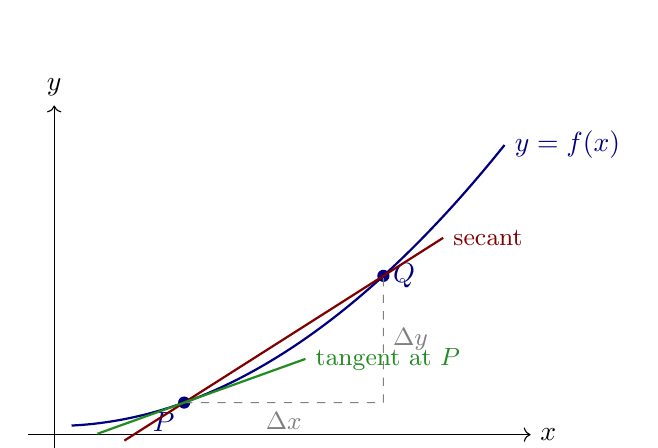
\begin{tikzpicture}[scale=1.1]
  % Axes
  \draw[->] (-0.3,0) -- (5.5,0) node[right]{$x$};
  \draw[->] (0,-0.3) -- (0,3.8) node[above]{$y$};
  % Curve
  \draw[thick,NavyBlue,domain=0.2:5.2,samples=80]
    plot(\x,{0.12*\x*\x + 0.1}) node[right]{$y=f(x)$};
  % Two points
  \coordinate (P) at (1.5,{0.12*1.5*1.5+0.1});
  \coordinate (Q) at (3.8,{0.12*3.8*3.8+0.1});
  \fill[NavyBlue] (P) circle(2pt) node[below left]{$P$};
  \fill[NavyBlue] (Q) circle(2pt) node[right]{$Q$};
  % Secant
  \draw[thick,Maroon] ($(P)!-0.3!(Q)$) -- ($(P)!1.3!(Q)$)
    node[right,Maroon]{\small secant};
  % Delta labels
  \draw[dashed,gray] (P) -- ({3.8},{0.12*1.5*1.5+0.1})
    node[midway,below]{\small $\Delta x$};
  \draw[dashed,gray] ({3.8},{0.12*1.5*1.5+0.1}) -- (Q)
    node[midway,right]{\small $\Delta y$};
  % Tangent at P
  \pgfmathsetmacro{\slope}{2*0.12*1.5}
  \draw[thick,ForestGreen]
    ({1.5-1},{\slope*(1.5-1-1.5)+0.12*1.5*1.5+0.1}) --
    ({1.5+1.4},{\slope*(1.5+1.4-1.5)+0.12*1.5*1.5+0.1})
    node[right,ForestGreen]{\small tangent at $P$};
\end{tikzpicture}
\caption{As $Q$ approaches $P$ along the curve, the secant line (Maroon)
rotates toward the tangent line (green). The limiting direction is the
derivative.}
\label{fig:secant-tangent}
\end{figure}

Now consider not a wall but a curve. A curve does not have a single slope; its
steepness varies from point to point. To measure its inclination at a single
location, we approximate it by secant lines connecting nearby points. As those
points approach one another, the secant line approaches a unique limiting line:
the tangent (\cref{fig:secant-tangent}).

The tangent line balances error symmetrically. It is the line for which
deviations on one side cancel those on the other to first order. This balancing
process resembles a lever in equilibrium: two equal perturbations placed
symmetrically about a point must balance to produce equilibrium.

Thus the derivative, at its core, is a \emph{local balance condition}. It is
the unique linear relation that stabilises infinitesimal variation.

\section{Limits as Stability Under Refinement}

The concept of limit formalises the idea of refinement. Suppose one estimates
the circumference of a circle by inscribing polygons with increasingly many
sides. As the number of sides increases, the perimeter approaches a fixed value.
One approaches the same number from above and below.

\begin{figure}[H]
\centering
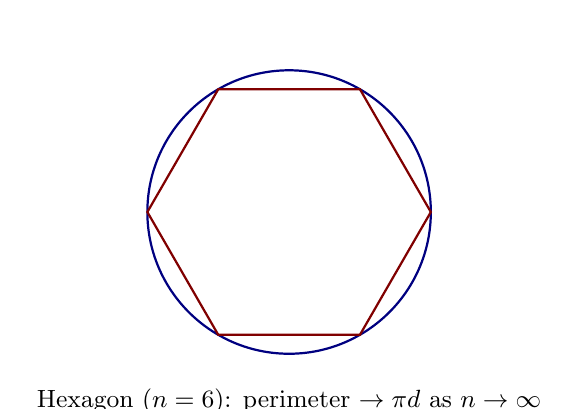
\begin{tikzpicture}[scale=1.2]
  \draw[thick,NavyBlue] (0,0) circle(1.5cm);
  % Inscribed hexagon
  \draw[Maroon,thick]
    (1.5,0) -- (0.75,1.299) -- (-0.75,1.299) --
    (-1.5,0) -- (-0.75,-1.299) -- (0.75,-1.299) -- cycle;
  % Inscribed triangle labels
  \node at (0,-2) {\small Hexagon ($n=6$): perimeter $\to \pi d$ as $n\to\infty$};
\end{tikzpicture}
\caption{Inscribed polygons approximate the circle's circumference. Convergence
is stability under refinement.}
\label{fig:polygon-limit}
\end{figure}

Convergence is not merely approximation—it is \emph{agreement under arbitrarily
small perturbation}.

\begin{definition}{Limit}{limit}
  A function $f(x)$ approaches $L$ as $x \to a$, written
  $\displaystyle\lim_{x\to a} f(x) = L$,
  if for every tolerance $\varepsilon > 0$ there exists $\delta > 0$ such that
  \[
    0 < |x - a| < \delta \implies |f(x) - L| < \varepsilon.
  \]
\end{definition}

This definition encodes stability. No matter how tightly one constrains
acceptable error, one can restrict attention sufficiently to guarantee
compliance. The limit is the expression of \emph{controlled variation}.

\begin{example}
  Let $f(x) = \frac{x^2 - 1}{x-1}$ for $x \neq 1$. Although $f$ is not
  defined at $x=1$, we compute
  $\lim_{x\to 1}\frac{x^2-1}{x-1} = \lim_{x\to 1}(x+1) = 2.$
  The limit captures the behaviour of $f$ near 1 without requiring evaluation
  at 1.
\end{example}

\section{The Derivative as a Sensitivity Operator}
\label{sec:deriv-sensitivity}

\begin{definition}{Derivative}{derivative}
  The derivative of $f:\R\to\R$ at $x$ is
  \[
    f'(x) = \lim_{h \to 0} \frac{f(x+h) - f(x)}{h},
  \]
  provided this limit exists.
\end{definition}

This expression measures how much $f$ responds to a small perturbation in $x$.
The numerator represents output change; the denominator represents input change;
their ratio is \emph{relational sensitivity}.

When the limit exists, $f$ is locally approximable by a linear map:
\[
  f(x + h) = f(x) + f'(x)h + o(h).
\]
The notation $o(h)$ means a term that vanishes faster than $h$ as $h\to 0$.

\begin{insight}
  The derivative is not merely a number. It is the coefficient of the best
  local linear model—the linear approximation that most faithfully captures
  the function's behaviour near a point.
\end{insight}

Constants vanish under differentiation because they exhibit no relational
sensitivity. Linear terms become constants because their deformation is uniform.
Higher-degree terms reduce degree because curvature itself varies. The
derivative strips away inert components and retains only those parts that
actively participate in change.

\begin{example}[Power rule]
  For $f(x) = x^n$ with $n \in \mathbb{Z}_{>0}$, the binomial theorem gives
  \[
    \frac{(x+h)^n - x^n}{h}
    = nx^{n-1} + \binom{n}{2}x^{n-2}h + \cdots \xrightarrow{h\to 0} nx^{n-1}.
  \]
  Thus $(x^n)' = nx^{n-1}$, the power rule.
\end{example}

\section{Abstraction as Reduction of Irrelevant Degrees of Freedom}

When differentiating
\[
  f(x) = ax^3 + bx^2 + cx + d,
\]
the result
\[
  f'(x) = 3ax^2 + 2bx + c
\]
reveals structure independent of arithmetic complication. The transformation
rule does not depend on the magnitude of $a$, $b$, $c$, $d$. It depends only
on exponentiation and linearity. Abstraction removes irrelevant degrees of
freedom while preserving relational form.

This principle recurs throughout the text. Calculus is not a collection of
tricks but a disciplined method for isolating structural relationships from
computational noise.

%% ═══════════════════════════════════════════════════════════════════════════
\chapter{Higher-Order Change and Curvature}
\label{ch:curvature}
%% ═══════════════════════════════════════════════════════════════════════════

\section{The Second Derivative and the Geometry of Bending}

The second derivative measures the rate at which the slope itself changes:
\[
  f''(x) = \frac{d}{dx}\bigl(f'(x)\bigr).
\]

\begin{figure}[H]
\centering
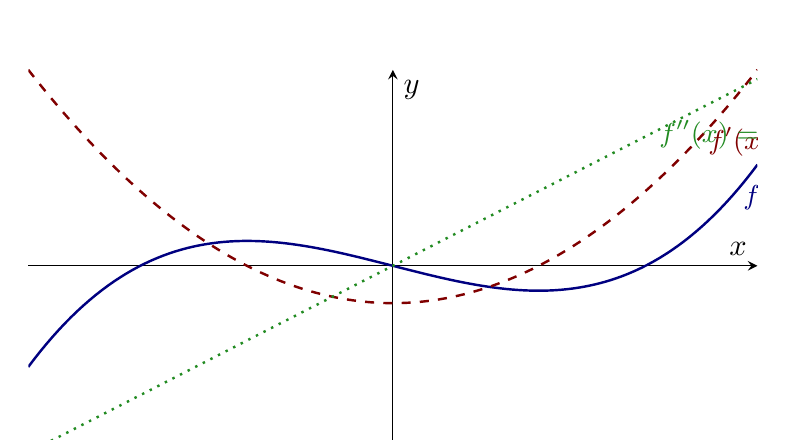
\begin{tikzpicture}[scale=1.1]
  \begin{axis}[
    width=10cm, height=6cm,
    axis lines=center,
    xlabel={$x$}, ylabel={$y$},
    samples=120, domain=-2.5:2.5,
    xtick=\empty, ytick=\empty,
    legend pos=north west,
    legend style={font=\small}
  ]
    \addplot[NavyBlue,thick]{x^3 - 3*x}
      node[right,pos=0.9,font=\small]{$f(x)=x^3-3x$};
    \addplot[Maroon,thick,dashed]{3*x^2 - 3}
      node[right,pos=0.85,font=\small]{$f'(x)=3x^2-3$};
    \addplot[ForestGreen,thick,dotted]{6*x}
      node[right,pos=0.85,font=\small]{$f''(x)=6x$};
  \end{axis}
\end{tikzpicture}
\caption{A function (blue), its first derivative (red dashed), and second
derivative (green dotted). Where $f''>0$ the function is concave up; where
$f''<0$ it is concave down.}
\label{fig:deriv-hierarchy}
\end{figure}

The Taylor expansion makes the role of the second derivative explicit:
\[
  f(x+h) = f(x) + f'(x)h + \frac{1}{2}f''(x)h^2 + o(h^2).
\]

The quadratic term encodes bending. It quantifies the deviation from perfect
linearity. Higher derivatives describe successive layers of structural
refinement: each derivative reveals how deformation itself deforms.

\section{Critical Points and Stability}

\begin{definition}{Critical point}{crit}
  A point $x_0$ is \emph{critical} for $f$ if $f'(x_0)=0$.
\end{definition}

Near a critical point,
\[
  f(x_0 + h) = f(x_0) + \tfrac{1}{2}f''(x_0)h^2 + o(h^2).
\]

Since $h^2 \ge 0$, the sign of $f''(x_0)$ determines whether perturbations
raise or lower the function.

\begin{theorem}{Second Derivative Test}{sdt}
  Let $f'(x_0)=0$.
  \begin{itemize}[leftmargin=1.5em]
    \item If $f''(x_0)>0$, then $x_0$ is a local minimum.
    \item If $f''(x_0)<0$, then $x_0$ is a local maximum.
    \item If $f''(x_0)=0$, the test is inconclusive.
  \end{itemize}
\end{theorem}

\begin{insight}
  Stability is a curvature condition. Positive curvature confines nearby
  trajectories; negative curvature repels them.
\end{insight}

\section{From One Variable to Many}

Real systems rarely depend on a single variable. For $f:\R^n\to\R$, each
coordinate may vary independently.

\begin{definition}{Partial derivative}{partial}
  The partial derivative of $f$ with respect to $x_i$ is
  \[
    \frac{\partial f}{\partial x_i}(x)
    = \lim_{h\to 0}
      \frac{f(x_1,\dots,x_i+h,\dots,x_n)-f(x)}{h}.
  \]
\end{definition}

Collecting all partial derivatives yields the \emph{gradient vector}:
\[
  \nabla f(x) =
  \begin{pmatrix}
    \partial f/\partial x_1 \\ \vdots \\ \partial f/\partial x_n
  \end{pmatrix}.
\]

The gradient is not a collection of slopes but a \emph{directional sensitivity
field}.

\section{Directional Derivatives and Linear Structure}

Let $v\in\R^n$ be a unit direction vector. The directional derivative is
\[
  D_v f(x) = \lim_{h\to 0}\frac{f(x+hv)-f(x)}{h}.
\]

When $f$ is differentiable,
\[
  D_v f(x) = \nabla f(x)\cdot v.
\]

The gradient therefore represents the \emph{linear functional} that maps
directional perturbations to scalar responses. Differentiability in
$\R^n$ means that $f$ admits a linear approximation:
\[
  f(x+h) = f(x) + \nabla f(x)\cdot h + o(\|h\|).
\]

\begin{figure}[H]
\centering
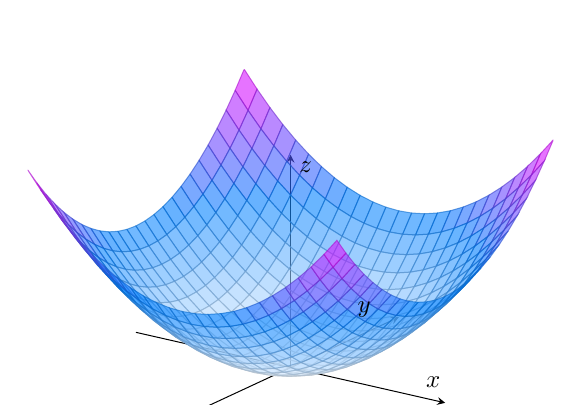
\begin{tikzpicture}[scale=0.9]
  \begin{axis}[
    view={35}{30},
    width=9cm, height=7cm,
    axis lines=center,
    xlabel={$x$}, ylabel={$y$}, zlabel={$z$},
    xtick=\empty, ytick=\empty, ztick=\empty,
    samples=25, domain=-2:2,
    colormap/cool
  ]
    \addplot3[surf,opacity=0.6]{x^2+y^2};
  \end{axis}
\end{tikzpicture}
\caption{The paraboloid $f(x,y)=x^2+y^2$. The gradient $\nabla f = (2x,2y)$
points radially outward — in the direction of steepest ascent — and is always
perpendicular to the level curves (circles).}
\label{fig:gradient}
\end{figure}

%% ═══════════════════════════════════════════════════════════════════════════
\chapter{Tangent Spaces and Local Models}
\label{ch:tangent}
%% ═══════════════════════════════════════════════════════════════════════════

\section{Curves and Embedded Surfaces}

At a point $p$ on a smooth surface $S\subset\R^3$, curves lying on $S$ have
velocity vectors at $p$. The collection of all such velocity vectors forms a
plane: the tangent plane.

\begin{figure}[H]
\centering
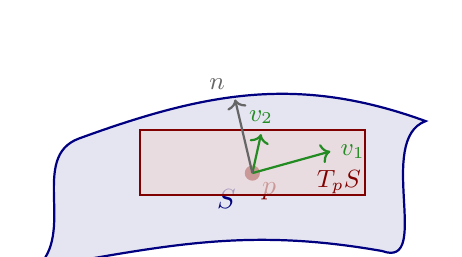
\begin{tikzpicture}[scale=1.1]
  % Draw a curved surface suggestively
  \fill[NavyBlue!10] (-2,-0.5) to[out=10,in=170] (2,-0.3)
    to[out=-20,in=200] (2.5,1.2) to[out=160,in=20] (-1.5,1.0)
    to[out=200,in=40] (-2,-0.5);
  \draw[thick,NavyBlue] (-2,-0.5) to[out=10,in=170] (2,-0.3)
    to[out=-20,in=200] (2.5,1.2) to[out=160,in=20] (-1.5,1.0)
    to[out=200,in=40] (-2,-0.5);
  \node[NavyBlue] at (0.2,0.3) {$S$};
  % Point p
  \coordinate (p) at (0.5,0.6);
  \fill[Maroon] (p) circle(2.5pt) node[below right]{$p$};
  % Tangent plane
  \fill[Maroon!15,opacity=0.7]
    (-0.8,0.35) -- (1.8,0.35) -- (1.8,1.1) -- (-0.8,1.1) -- cycle;
  \draw[Maroon,thick]
    (-0.8,0.35) -- (1.8,0.35) -- (1.8,1.1) -- (-0.8,1.1) -- cycle;
  \node[Maroon] at (1.5,0.5) {\small $T_p S$};
  % Tangent vectors
  \draw[->,thick,ForestGreen] (p) -- ++(0.9,0.25)
    node[right,ForestGreen,font=\small]{$v_1$};
  \draw[->,thick,ForestGreen] (p) -- ++(0.1,0.45)
    node[above,ForestGreen,font=\small]{$v_2$};
  % Normal
  \draw[->,thick,black!60] (p) -- ++(-0.2,0.85)
    node[above left,font=\small]{$n$};
\end{tikzpicture}
\caption{The tangent space $T_p S$ (red plane) at a point $p$ on a surface $S$
(blue). Tangent vectors $v_1,v_2$ lie in the plane; the normal $n$ is
perpendicular to it.}
\label{fig:tangent-space}
\end{figure}

\begin{definition}{Tangent space of a manifold}{tangentspace}
  For a smooth manifold $M$ and a point $x\in M$, the tangent space is
  \[
    T_x M = \bigl\{\gamma'(0) \mid
      \gamma:(-\varepsilon,\varepsilon)\to M,\; \gamma(0)=x \bigr\}.
  \]
  The tangent space captures all possible instantaneous directions of motion
  constrained to $M$.
\end{definition}

\section{Functions Between Manifolds and the Jacobian}

Let $F:M\to N$ be a smooth map between manifolds. The derivative of $F$ at $x$
is the linear map
\[
  dF_x : T_x M \to T_{F(x)} N.
\]

For $F:\R^n\to\R^m$, this linear map is represented by the Jacobian matrix:
\[
  J_F(x) =
  \begin{pmatrix}
    \dfrac{\partial F_1}{\partial x_1} & \cdots &
    \dfrac{\partial F_1}{\partial x_n} \\[8pt]
    \vdots & \ddots & \vdots \\[4pt]
    \dfrac{\partial F_m}{\partial x_1} & \cdots &
    \dfrac{\partial F_m}{\partial x_n}
  \end{pmatrix}.
\]

The Jacobian is the multivariable generalisation of slope.

\section{The Chain Rule as Composition of Deformation}

\begin{theorem}{Chain Rule}{chain}
  For smooth maps $F:M\to N$ and $G:N\to P$,
  \[
    d(G\circ F)_x = dG_{F(x)}\circ dF_x.
  \]
\end{theorem}

The derivative of a composition is the composition of derivatives. In
coordinates:
\[
  J_{G\circ F}(x) = J_G(F(x))\cdot J_F(x).
\]

\begin{insight}
  The chain rule is not computational coincidence; it is a categorical necessity
  of linear approximation. Local deformation in $M$ maps into $N$, then into
  $P$. Sensitivity composes.
\end{insight}

\begin{figure}[H]
\centering
\begin{tikzcd}[column sep=3em, row sep=2em]
  T_x M \arrow[r,"dF_x"] \arrow[dr,swap,"d(G\circ F)_x"]
  & T_{F(x)} N \arrow[d,"dG_{F(x)}"] \\
  & T_{(G\circ F)(x)} P
\end{tikzcd}
\caption{The chain rule as commutative diagram: the composite derivative equals
the composition of individual derivatives.}
\label{fig:chain-cd}
\end{figure}

\section{The Hessian and Second-Order Structure}

For $f:\R^n\to\R$, the second derivative is encoded in the Hessian matrix:
\[
  H_f(x) = \Bigl(\frac{\partial^2 f}{\partial x_i\partial x_j}\Bigr)_{i,j}.
\]

The quadratic Taylor expansion is
\[
  f(x+h) = f(x) + \nabla f(x)\cdot h + \tfrac{1}{2}h^\top H_f(x)h + o(\|h\|^2).
\]

\begin{theorem}{Multivariable Second Derivative Test}{mvarsdt}
  Let $\nabla f(x_0)=0$. Stability at $x_0$ is determined by the eigenvalues of
  $H_f(x_0)$:
  \begin{itemize}[leftmargin=1.5em]
    \item All eigenvalues positive $\Rightarrow$ local minimum.
    \item All eigenvalues negative $\Rightarrow$ local maximum.
    \item Mixed signs $\Rightarrow$ saddle point.
  \end{itemize}
\end{theorem}

%% ═══════════════════════════════════════════════════════════════════════════
\chapter{Integration and Reconstruction}
\label{ch:integration}
%% ═══════════════════════════════════════════════════════════════════════════

\section{Accumulation from Infinitesimal Influence}

If the derivative measures how a quantity changes locally, the integral measures
how local changes accumulate into global structure. The two operations are
inverse procedures within a unified stability framework.

\begin{figure}[H]
\centering
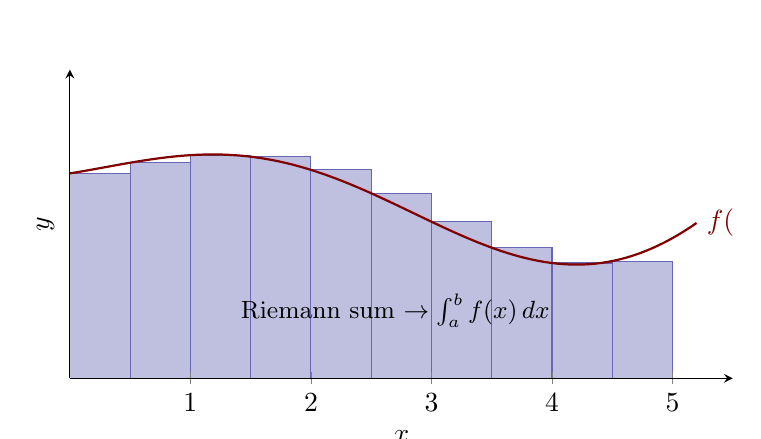
\begin{tikzpicture}[scale=1.0]
  \begin{axis}[
    width=10cm, height=5.5cm,
    axis lines=left,
    xlabel={$x$}, ylabel={$y$},
    xmin=0, xmax=5.5, ymin=0, ymax=3.2,
    xtick={1,2,3,4,5},
    ytick=\empty,
    samples=100,
    area style
  ]
    % Shaded Riemann sum
    \addplot[ybar interval, fill=NavyBlue!25, draw=NavyBlue!60,
      samples at={0,0.5,1,1.5,2,2.5,3,3.5,4,4.5,5}]
      {0.1*(x-2.5)^2 + 0.7*sin(deg(x))+1.5};
    % True function on top
    \addplot[thick,Maroon,domain=0:5.2]
      {0.1*(x-2.5)^2 + 0.7*sin(deg(x))+1.5}
      node[right]{$f(x)$};
    \node at (2.7,0.7) {\small Riemann sum $\to \int_a^b f(x)\,dx$};
  \end{axis}
\end{tikzpicture}
\caption{A Riemann sum (blue rectangles) approximating the integral of $f$ over
$[0,5]$. As rectangle widths shrink to zero, the sum converges to the definite
integral.}
\label{fig:riemann}
\end{figure}

\begin{definition}{Definite integral}{defint}
  If $f:[a,b]\to\R$ and the Riemann sums
  \[
    S_n = \sum_{i=0}^{n-1} f(x_i^*)\,\Delta x_i
  \]
  converge as $\max_i \Delta x_i\to 0$ (independently of the choice of sample
  points), the limit is the \emph{definite integral}
  \[
    \int_a^b f(x)\,dx.
  \]
\end{definition}

\section{The Fundamental Theorem of Calculus}

\begin{theorem}{Fundamental Theorem of Calculus}{ftc}
  Let $f$ be continuous on $[a,b]$.
  \begin{enumerate}[label=(\roman*)]
    \item If $F(x) = \int_a^x f(t)\,dt$, then $F'(x) = f(x)$.
    \item If $F'(x)=f(x)$, then $\int_a^b f(x)\,dx = F(b)-F(a)$.
  \end{enumerate}
\end{theorem}

\begin{insight}
  The Fundamental Theorem is not merely computational convenience. It expresses
  that global structure can be reconstructed from local sensitivity, and local
  sensitivity can be extracted from global structure. The integral aggregates
  deformation; the derivative isolates it.
\end{insight}

\begin{proof}[Proof sketch of Part (i)]
  By definition,
  $F'(x) = \lim_{h\to 0}\frac{1}{h}\int_x^{x+h}f(t)\,dt.$
  By continuity of $f$, for any $\varepsilon>0$ there exists $\delta>0$ such
  that $|f(t)-f(x)|<\varepsilon$ whenever $|t-x|<\delta$. Then
  \[
    \left|\frac{1}{h}\int_x^{x+h}f(t)\,dt - f(x)\right|
    = \left|\frac{1}{h}\int_x^{x+h}(f(t)-f(x))\,dt\right|
    \le \varepsilon.
  \]
  Since $\varepsilon$ was arbitrary, $F'(x)=f(x)$.
\end{proof}

\section{Change of Variables and Structural Invariance}

For a transformation $x=g(u)$:
\[
  \int f(x)\,dx = \int f(g(u))\,g'(u)\,du.
\]

In multiple dimensions, if $\Phi:\R^n\to\R^n$ is smooth with Jacobian
determinant $\det J_\Phi$, then
\[
  \int_{\Phi(U)} h(x)\,dx = \int_U h(\Phi(u))\,|\det J_\Phi(u)|\,du.
\]

The Jacobian determinant measures how \emph{volume scales} under the
transformation. Integration must incorporate this geometric correction to remain
invariant.

\begin{example}[Polar coordinates]
  The transformation $x=r\cos\theta$, $y=r\sin\theta$ has
  $\det J = r$, giving the familiar formula
  $\iint_\Omega f(x,y)\,dx\,dy = \int_0^{2\pi}\int_0^R f(r\cos\theta,
  r\sin\theta)\,r\,dr\,d\theta.$
\end{example}

%% ═══════════════════════════════════════════════════════════════════════════
\chapter{Differential Equations and Dynamics}
\label{ch:ode}
%% ═══════════════════════════════════════════════════════════════════════════

\section{Rates as Laws of Motion}

A differential equation prescribes how a quantity evolves in response to its
current state. It defines a rule of motion rather than a static relationship.

\begin{definition}{Ordinary differential equation}{ode}
  A first-order ODE is an equation of the form
  \[
    \frac{dx}{dt} = f(x,t),
  \]
  where $x:\R\to\R$ (or $\R^n$) is unknown and $f$ specifies instantaneous
  rate of change.
\end{definition}

Solving a differential equation means \emph{reconstructing global behaviour
from a local law}.

\begin{figure}[H]
\centering
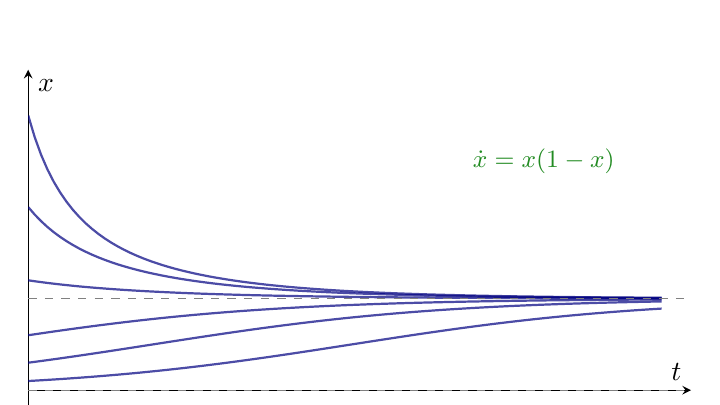
\begin{tikzpicture}[scale=1.0]
  \begin{axis}[
    width=10cm, height=6cm,
    axis lines=center,
    xlabel={$t$}, ylabel={$x$},
    xmin=0, xmax=4.5, ymin=-0.3, ymax=3.5,
    xtick=\empty, ytick=\empty,
    samples=100
  ]
    % Several solution curves for dx/dt = x(1-x)
    \foreach \xinit in {0.1,0.3,0.6,1.2,2.0,3.0}{
      \addplot[NavyBlue,thick,domain=0:4.3,opacity=0.7]
        {1/(1+(1/\xinit - 1)*exp(-x))};
    }
    % Label equilibria
    \draw[dashed,gray] (0,1) -- (4.5,1) node[right,gray]{\small $x=1$};
    \draw[dashed,gray] (0,0) -- (4.5,0) node[right,gray]{\small $x=0$};
    \node[ForestGreen] at (3.5,2.5) {\small $\dot x = x(1-x)$};
  \end{axis}
\end{tikzpicture}
\caption{Phase portrait for the logistic equation $\dot x = x(1-x)$. All
trajectories with $x(0)>0$ converge to $x=1$ (stable equilibrium); $x=0$ is
unstable.}
\label{fig:logistic}
\end{figure}

\section{Equilibria and Linearisation}

An equilibrium $x_0$ satisfies $f(x_0)=0$. Near equilibrium, a Taylor
expansion gives the \emph{linearised equation}:
\[
  \frac{d}{dt}(x-x_0) = f'(x_0)(x-x_0) + \text{higher-order terms}.
\]

\begin{theorem}{Stability via linearisation}{stablin}
  Let $x_0$ be an equilibrium of $\dot x = f(x)$.
  \begin{itemize}[leftmargin=1.5em]
    \item If $f'(x_0)<0$, perturbations decay exponentially; $x_0$ is
      \emph{asymptotically stable}.
    \item If $f'(x_0)>0$, perturbations grow; $x_0$ is \emph{unstable}.
  \end{itemize}
\end{theorem}

In higher dimensions, stability depends on the eigenvalues of $J_f(x_0)$.

\section{Systems of Differential Equations}

For $x\in\R^n$, the system $\dot x = F(x)$ defines a \emph{vector field} on
state space. Each initial condition generates a trajectory determined by the
integral curves of $F$.

For linear systems $\dot x = Ax$, the solution is
\[
  x(t) = e^{At}x(0),
\]
where $e^{At}$ is the matrix exponential. The eigenvalues of $A$ determine
long-term behaviour:
\begin{itemize}[leftmargin=1.5em]
  \item Negative real parts $\Rightarrow$ exponential decay.
  \item Positive real parts $\Rightarrow$ exponential growth.
  \item Purely imaginary parts $\Rightarrow$ oscillation.
\end{itemize}

\begin{figure}[H]
\centering
\begin{tikzpicture}[scale=0.85]
  % Stable node (left)
  \begin{scope}[xshift=0cm]
    \draw[->] (-2.3,0)--(2.3,0) node[right,font=\small]{$x_1$};
    \draw[->] (0,-2.3)--(0,2.3) node[above,font=\small]{$x_2$};
    \node[font=\small] at (0,2.6) {Stable node};
    \foreach \x in {-1.5,-0.7,0.7,1.5}{
      \foreach \y in {-1.5,-0.7,0.7,1.5}{
        \pgfmathsetmacro{\vx}{-\x}
        \pgfmathsetmacro{\vy}{-2*\y}
        \pgfmathsetmacro{\mag}{sqrt(\vx*\vx+\vy*\vy)+0.001}
        \draw[->,NavyBlue!70,thin]
          (\x,\y) -- ({\x+0.3*\vx/\mag},{\y+0.3*\vy/\mag});
      }
    }
  \end{scope}
  % Saddle point (right)
  \begin{scope}[xshift=6cm]
    \draw[->] (-2.3,0)--(2.3,0) node[right,font=\small]{$x_1$};
    \draw[->] (0,-2.3)--(0,2.3) node[above,font=\small]{$x_2$};
    \node[font=\small] at (0,2.6) {Saddle point};
    \foreach \x in {-1.5,-0.7,0.7,1.5}{
      \foreach \y in {-1.5,-0.7,0.7,1.5}{
        \pgfmathsetmacro{\vx}{\x}
        \pgfmathsetmacro{\vy}{-\y}
        \pgfmathsetmacro{\mag}{sqrt(\vx*\vx+\vy*\vy)+0.001}
        \draw[->,Maroon!70,thin]
          (\x,\y) -- ({\x+0.3*\vx/\mag},{\y+0.3*\vy/\mag});
      }
    }
  \end{scope}
\end{tikzpicture}
\caption{Phase portraits for a stable node (left, both eigenvalues negative)
and a saddle point (right, eigenvalues of opposite sign).}
\label{fig:phase-portraits}
\end{figure}

%% ═══════════════════════════════════════════════════════════════════════════
\chapter{Curvature, Constraint, and Manifolds}
\label{ch:manifolds}
%% ═══════════════════════════════════════════════════════════════════════════

\section{Motion Under Constraint}

If motion is restricted to a manifold $M$, the differential equation becomes
\[
  \frac{dx}{dt} = \proj{T_x M} F(x),
\]
where $\proj{T_x M}$ denotes orthogonal projection onto the tangent space.
This ensures trajectories remain on the manifold by suppressing normal
components (\cref{fig:tangent-space}).

\begin{example}[Pendulum]
  A pendulum of length $\ell$ is constrained to the circle of radius $\ell$.
  The unconstrained gravity vector is projected onto the tangential direction,
  yielding $\ddot\theta = -(g/\ell)\sin\theta$.
\end{example}

\section{Curvature and Geodesics}

On a Riemannian manifold $(M,g)$, geodesics are curves that locally minimise
length. They satisfy the geodesic equation
\[
  \nabla_{\dot\gamma}\dot\gamma = 0,
\]
where $\nabla$ is the Levi-Civita connection.

\begin{figure}[H]
\centering
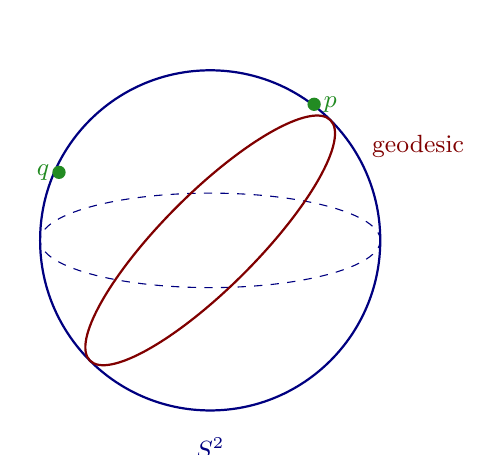
\begin{tikzpicture}[scale=1.2]
  % Sphere sketch
  \draw[NavyBlue,thick] (0,0) circle(1.8cm);
  \draw[NavyBlue,dashed] (0,0) ellipse(1.8cm and 0.5cm);
  % Great circle (geodesic)
  \draw[Maroon,thick,rotate=45]
    (0,0) ellipse(1.8cm and 0.5cm);
  \node[Maroon] at (2.2,1.0) {\small geodesic};
  % Two points
  \fill[ForestGreen] (1.1,1.44) circle(2pt) node[right,ForestGreen,font=\small]{$p$};
  \fill[ForestGreen] (-1.6,0.72) circle(2pt) node[left,ForestGreen,font=\small]{$q$};
  \node[NavyBlue] at (0,-2.2) {\small $S^2$};
\end{tikzpicture}
\caption{A geodesic (great circle) on the sphere $S^2$ connecting points $p$
and $q$. The geodesic minimises length; curvature causes geodesics to converge
at poles.}
\label{fig:geodesic}
\end{figure}

The \emph{Riemann curvature tensor} $R$ measures how geodesics initially
parallel deviate from one another under parallel transport. Positive curvature
(as on a sphere) causes convergence; negative curvature (as on a hyperbolic
surface) causes divergence.

\section{The Structural Unity of Calculus}

The themes developed in the first six chapters can be summarised in a single
diagram:

\begin{figure}[H]
\centering
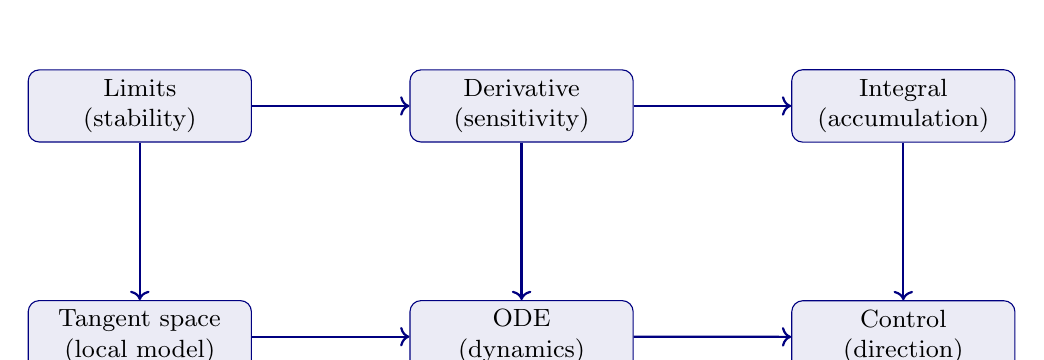
\begin{tikzpicture}[
  node distance=2.0cm,
  box/.style={rectangle,rounded corners,draw=NavyBlue,fill=NavyBlue!8,
              text width=2.6cm,align=center,font=\small},
  arr/.style={->,thick,NavyBlue}
]
  \node[box] (limit)   {Limits\\(stability)};
  \node[box,right=of limit] (deriv)   {Derivative\\(sensitivity)};
  \node[box,right=of deriv] (integral){Integral\\(accumulation)};
  \node[box,below=of deriv] (ode)     {ODE\\(dynamics)};
  \node[box,below=of limit] (tangent) {Tangent space\\(local model)};
  \node[box,below=of integral] (control){Control\\(direction)};

  \draw[arr] (limit) -- (deriv);
  \draw[arr] (deriv) -- (integral);
  \draw[arr] (deriv) -- (ode);
  \draw[arr] (tangent) -- (ode);
  \draw[arr] (ode) -- (control);
  \draw[arr] (limit) -- (tangent);
  \draw[arr] (integral) -- (control);
\end{tikzpicture}
\caption{Structural dependencies among the core concepts of calculus.}
\label{fig:calculus-map}
\end{figure}

%% ═══════════════════════════════════════════════════════════════════════════
\chapter{Multivariable Integration Theory}
\label{ch:multint}
%% ═══════════════════════════════════════════════════════════════════════════

\section{Measure and Volume in Higher Dimensions}

For a bounded region $\Omega\subset\R^n$, the integral of $f:\Omega\to\R$
is defined by partitioning into small subregions of volume $\Delta V_i$:
\[
  \int_\Omega f(x)\,dx
  = \lim_{\max\Delta V_i\to 0} \sum_i f(x_i^*)\,\Delta V_i.
\]

\section{Iterated Integrals and Fubini's Theorem}

\begin{theorem}{Fubini}{fubini}
  If $f:\Omega\to\R$ is integrable on $\Omega=[a,b]\times[c,d]$, then
  \[
    \int_\Omega f(x,y)\,dx\,dy
    = \int_a^b\!\!\int_c^d f(x,y)\,dy\,dx
    = \int_c^d\!\!\int_a^b f(x,y)\,dx\,dy.
  \]
\end{theorem}

The significance is structural: accumulation along independent coordinate
directions is compatible with accumulation over the whole region. Volume measure
factorises across orthogonal directions.

\section{Coordinate Transformations and the Jacobian Determinant}

For a smooth bijection $\Phi:U\to\Omega$,
\[
  \int_\Omega f(x)\,dx
  = \int_U f(\Phi(u))\,|\det D\Phi(u)|\,du.
\]

The Jacobian determinant measures local volume distortion. It is the net scaling
factor of the linear map $D\Phi(u)$, capturing how infinitesimal cubes deform
under the transformation.

\section{Integration over Curves and Surfaces}

For a smooth curve $\gamma:[a,b]\to\R^n$, the arc-length integral is
\[
  \int_\gamma f\,ds
  = \int_a^b f(\gamma(t))\,\|\gamma'(t)\|\,dt.
\]

For a surface $S$ parameterised by $\Phi(u,v)$:
\[
  \int_S f\,dS
  = \int_U f(\Phi(u,v))\,
    \|\partial_u\Phi\times\partial_v\Phi\|\,du\,dv.
\]

In both cases: integration equals \emph{accumulation of infinitesimal geometric
elements weighted by local density}.

\section{Orientation and Differential Forms}

A differential $k$-form assigns oriented infinitesimal $k$-dimensional volume
elements to tangent spaces. Orientation determines the sign of accumulated
quantities. The exterior derivative $d$ maps $k$-forms to $(k+1)$-forms and
satisfies $d^2=0$, encoding the fact that \emph{boundaries of boundaries
vanish}.

%% ═══════════════════════════════════════════════════════════════════════════
\chapter{Vector Calculus and the Geometry of Fields}
\label{ch:vecalc}
%% ═══════════════════════════════════════════════════════════════════════════

\section{Gradient, Divergence, and Curl}

Three differential operators play central roles in vector calculus.

\begin{definition}{Divergence}{divergence}
  For $F:\R^3\to\R^3$,
  \[
    \nabla\cdot F
    = \frac{\partial F_1}{\partial x}
    + \frac{\partial F_2}{\partial y}
    + \frac{\partial F_3}{\partial z}.
  \]
  Divergence measures local volumetric expansion ($\nabla\cdot F>0$) or
  compression ($\nabla\cdot F<0$).
\end{definition}

\begin{definition}{Curl}{curl}
  \[
    \nabla\times F
    = \begin{pmatrix}
        \partial_y F_3 - \partial_z F_2 \\
        \partial_z F_1 - \partial_x F_3 \\
        \partial_x F_2 - \partial_y F_1
      \end{pmatrix}.
  \]
  Curl measures local rotation density.
\end{definition}

\begin{figure}[H]
\centering
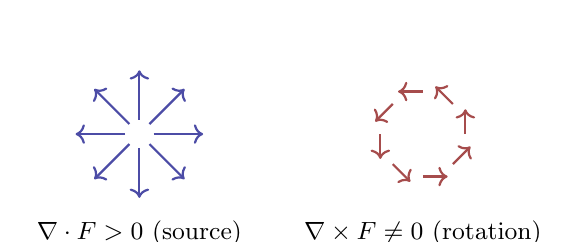
\begin{tikzpicture}[scale=0.9]
  % Diverging field
  \begin{scope}
    \foreach \angle in {0,45,...,315}{
      \draw[->,NavyBlue!70,thick]
        ({0.2*cos(\angle)},{0.2*sin(\angle)}) --
        ({0.9*cos(\angle)},{0.9*sin(\angle)});
    }
    \node at (0,-1.4) {\small $\nabla\cdot F>0$\ (source)};
  \end{scope}
  % Rotating field
  \begin{scope}[xshift=4cm]
    \foreach \angle in {0,45,...,315}{
      \draw[->,Maroon!70,thick]
        ({0.6*cos(\angle)},{0.6*sin(\angle)}) --
        ({0.6*cos(\angle)-0.35*sin(\angle)},
         {0.6*sin(\angle)+0.35*cos(\angle)});
    }
    \node at (0,-1.4) {\small $\nabla\times F\neq 0$\ (rotation)};
  \end{scope}
\end{tikzpicture}
\caption{Left: a diverging field with positive divergence (source). Right: a
rotating field with nonzero curl.}
\label{fig:div-curl}
\end{figure}

\section{The Divergence Theorem and Stokes' Theorem}

\begin{theorem}{Divergence Theorem}{divthm}
  For a region $\Omega$ with outward-pointing boundary normal $n$,
  \[
    \int_\Omega \nabla\cdot F\,dV
    = \int_{\partial\Omega} F\cdot n\,dS.
  \]
  Total interior expansion equals boundary flux.
\end{theorem}

\begin{theorem}{Stokes' Theorem}{stokes}
  For an oriented surface $S$ with boundary $\partial S$,
  \[
    \int_S (\nabla\times F)\cdot n\,dS
    = \int_{\partial S} F\cdot dr.
  \]
  Total curl over a surface equals boundary circulation.
\end{theorem}

Both theorems are special cases of the general Stokes theorem for differential
forms:
\[
  \int_{\partial M} \omega = \int_M d\omega.
\]
Boundary behaviour reflects interior variation. This is the geometric
expression of conservation laws.

%% ═══════════════════════════════════════════════════════════════════════════
\chapter{Nonlinear Dynamics and Phase Space}
\label{ch:nonlinear}
%% ═══════════════════════════════════════════════════════════════════════════

\section{Phase Portraits and Flow Geometry}

A nonlinear dynamical system
\[
  \frac{dx}{dt} = F(x), \qquad F:\R^n\to\R^n,
\]
assigns to each state an instantaneous direction of evolution. The collection
of all trajectories forms the \emph{flow} of the system.

\begin{figure}[H]
\centering
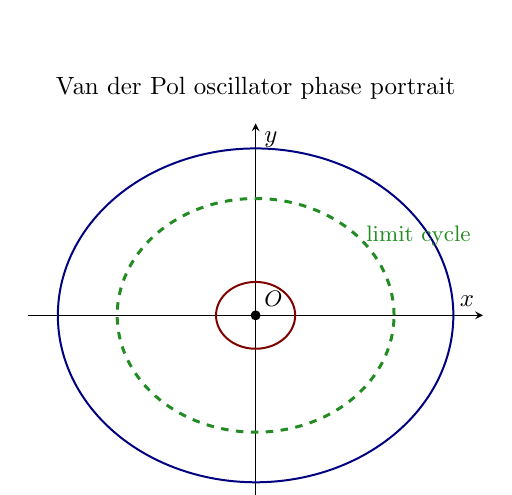
\begin{tikzpicture}[scale=0.9]
  \begin{axis}[
    width=8cm, height=7cm,
    axis lines=center,
    xlabel={$x$}, ylabel={$y$},
    xmin=-2.3, xmax=2.3, ymin=-2.3, ymax=2.3,
    xtick=\empty, ytick=\empty,
    title={Van der Pol oscillator phase portrait}
  ]
    % Several trajectories (approximate spiral inward to limit cycle)
    \addplot[NavyBlue,thick,domain=0:6.28,samples=200]
      ({2*cos(deg(x))}, {2*sin(deg(x))});
    \addplot[Maroon,thick,domain=0:6.28,samples=200]
      ({0.4*cos(deg(x))}, {0.4*sin(deg(x))});
    % Limit cycle
    \addplot[ForestGreen,very thick,dashed,domain=0:6.28,samples=200]
      ({1.4*cos(deg(x))},{1.4*sin(deg(x))})
      node[right,pos=0.12,font=\small,ForestGreen]{limit cycle};
    % Origin
    \fill (0,0) circle(2pt) node[above right,font=\small]{$O$};
  \end{axis}
\end{tikzpicture}
\caption{Schematic phase portrait of a limit cycle system. Trajectories
starting far out (blue) spiral inward; trajectories starting near the origin
(red) spiral outward. Both converge to the limit cycle (green dashed circle).}
\label{fig:limitcycle}
\end{figure}

\section{The Hartman--Grobman Theorem}

\begin{theorem}{Hartman--Grobman}{hg}
  If $x_0$ is a hyperbolic equilibrium of $\dot x = F(x)$ (i.e.\ no
  eigenvalue of $DF(x_0)$ lies on the imaginary axis), then the nonlinear
  system near $x_0$ is \emph{topologically conjugate} to its linearisation
  $\dot y = DF(x_0)\,y$.
\end{theorem}

Thus, near hyperbolic equilibria, nonlinear dynamics inherit qualitative
behaviour from linear systems. The eigenvalues of $DF(x_0)$ give a complete
local portrait.

\section{Lyapunov Functions and Energy Methods}

\begin{definition}{Lyapunov function}{lyapunov}
  A smooth function $V:\R^n\to\R_{\ge 0}$ is a Lyapunov function for
  $\dot x=F(x)$ at equilibrium $x_0$ if $V(x_0)=0$, $V(x)>0$ for $x\neq x_0$
  nearby, and $\dot V(x) := \nabla V(x)\cdot F(x) \le 0$ along trajectories.
\end{definition}

\begin{theorem}{Lyapunov stability}{lyapstab}
  If a Lyapunov function $V$ exists with $\dot V<0$ (strict), then $x_0$ is
  asymptotically stable.
\end{theorem}

Lyapunov functions generalise potential functions to non-conservative systems.
They provide stability certificates without requiring explicit solution of the
differential equation.

\section{Bifurcation Theory}

As a parameter $\mu$ varies, equilibria may appear, disappear, or change
stability. This is a \emph{bifurcation}.

\begin{example}[Pitchfork bifurcation]
  Consider $\dot x = \mu x - x^3$. For $\mu<0$, the only equilibrium is $x=0$
  (stable). For $\mu>0$, the origin becomes unstable and two new stable
  equilibria $x=\pm\sqrt{\mu}$ emerge (\cref{fig:pitchfork}).
\end{example}

\begin{figure}[H]
\centering
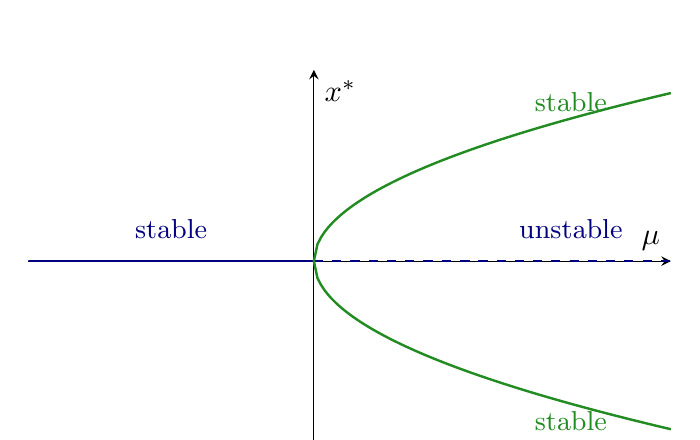
\begin{tikzpicture}[scale=1.1]
  \begin{axis}[
    width=9cm, height=6cm,
    axis lines=center,
    xlabel={$\mu$}, ylabel={$x^*$},
    xmin=-2, xmax=2.5, ymin=-1.8, ymax=1.8,
    xtick=\empty, ytick=\empty,
    samples=100
  ]
    % Stable branch for mu<0
    \addplot[NavyBlue,thick,domain=-2:0]{0};
    % Unstable branch for mu>0
    \addplot[NavyBlue,dashed,thick,domain=0:2.5]{0};
    % New stable branches
    \addplot[ForestGreen,thick,domain=0:2.5]{sqrt(x)};
    \addplot[ForestGreen,thick,domain=0:2.5]{-sqrt(x)};
    \node[NavyBlue] at (-1.0,0.3) {\small stable};
    \node[NavyBlue] at (1.8,0.3) {\small unstable};
    \node[ForestGreen] at (1.8,1.5) {\small stable};
    \node[ForestGreen] at (1.8,-1.5) {\small stable};
  \end{axis}
\end{tikzpicture}
\caption{Bifurcation diagram for the pitchfork bifurcation $\dot x=\mu x-x^3$.
At $\mu=0$, one stable equilibrium splits into three.}
\label{fig:pitchfork}
\end{figure}

%% ═══════════════════════════════════════════════════════════════════════════
\chapter{Constrained Dynamics and Lagrangian Structure}
\label{ch:lagrange}
%% ═══════════════════════════════════════════════════════════════════════════

\section{Variational Principles and the Euler--Lagrange Equation}

The calculus of variations generalises optimisation from functions to
\emph{functionals}.

\begin{definition}{Action functional}{action}
  Given a Lagrangian $L(q,\dot q,t)$, the action is
  \[
    \mathcal{S}[\gamma] = \int_a^b L(\gamma(t),\dot\gamma(t),t)\,dt.
  \]
\end{definition}

\begin{theorem}{Euler--Lagrange equation}{el}
  Critical curves of $\mathcal{S}$ satisfy
  \[
    \frac{d}{dt}\frac{\partial L}{\partial\dot\gamma}
    - \frac{\partial L}{\partial\gamma} = 0.
  \]
\end{theorem}

This equation arises by demanding that the first-order variation of the action
vanishes under all compactly supported perturbations. Motion becomes a
\emph{stationary condition} in function space.

\begin{insight}
  The Euler--Lagrange equation expresses dynamics as extremisation of accumulated
  quantities. Geodesics, classical trajectories, and elastica are all solutions
  to variational problems.
\end{insight}

\section{Hamiltonian Systems}

Define conjugate momentum $p=\partial L/\partial\dot q$ and Hamiltonian
\[
  H(q,p) = p\cdot\dot q - L.
\]

\begin{theorem}{Hamilton's equations}{hamilton}
  \[
    \dot q = \frac{\partial H}{\partial p}, \qquad
    \dot p = -\frac{\partial H}{\partial q}.
  \]
\end{theorem}

Hamiltonian flows preserve the symplectic form $\omega=dp\wedge dq$ and, when
$H$ is time-independent, conserve energy. Phase space volume is also conserved
(Liouville's theorem).

\section{Noether's Theorem}

\begin{theorem}{Noether}{noether}
  If the action $\mathcal{S}$ is invariant under a one-parameter family of
  transformations generated by a vector field $X$, then the quantity
  \[
    Q = \frac{\partial L}{\partial\dot\gamma}\cdot X(\gamma)
  \]
  is conserved along solutions.
\end{theorem}

Symmetry generates conservation. Temporal invariance gives energy conservation;
spatial translational invariance gives momentum conservation; rotational
invariance gives angular momentum conservation.

%% ═══════════════════════════════════════════════════════════════════════════
\chapter{Geometric Control Theory}
\label{ch:control}
%% ═══════════════════════════════════════════════════════════════════════════

\section{Control Systems as Vector Fields with Input}

A control system extends a dynamical system by introducing external inputs:
\[
  \frac{dx}{dt} = F(x) + \sum_{i=1}^m u_i\,G_i(x),
\]
where $F$ is the drift field, $G_i$ are control vector fields, and $u_i(t)$
are chosen inputs. Control introduces \emph{directed deformation}.

\section{Controllability and Lie Brackets}

\begin{definition}{Lie bracket}{liebracket}
  For smooth vector fields $X,Y$ on $\R^n$, the Lie bracket is
  \[
    [X,Y](x) = DY(x)\,X(x) - DX(x)\,Y(x).
  \]
\end{definition}

Lie brackets represent second-order motion generated by alternating flows.
Physically, flowing along $X$ for time $\sqrt{h}$, then $Y$, then $-X$, then
$-Y$ produces a displacement of order $h$ in direction $[X,Y]$.

\begin{theorem}{Chow--Rashevskii (accessibility)}{chow}
  If the distribution generated by $\{G_1,\dots,G_m\}$ and all their iterated
  Lie brackets spans $T_x\R^n$ at every $x$, then the system is
  \emph{accessible} (reachable from any point to any other).
\end{theorem}

\begin{figure}[H]
\centering
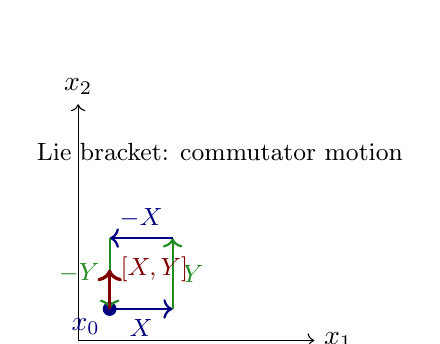
\begin{tikzpicture}[scale=1.0]
  \draw[->] (0,0) -- (3,0) node[right]{$x_1$};
  \draw[->] (0,0) -- (0,3) node[above]{$x_2$};
  % Start point
  \fill[NavyBlue] (0.4,0.4) circle(2.5pt) node[below left]{$x_0$};
  % Bracket loop
  \draw[->,thick,NavyBlue] (0.4,0.4) -- (1.2,0.4)
    node[midway,below,font=\small]{$X$};
  \draw[->,thick,ForestGreen] (1.2,0.4) -- (1.2,1.3)
    node[midway,right,font=\small]{$Y$};
  \draw[->,thick,NavyBlue] (1.2,1.3) -- (0.4,1.3)
    node[midway,above,font=\small]{$-X$};
  \draw[->,thick,ForestGreen] (0.4,1.3) -- (0.4,0.4)
    node[midway,left,font=\small]{$-Y$};
  % Residual direction [X,Y]
  \draw[->,very thick,Maroon] (0.4,0.4) -- (0.4,0.9)
    node[right,font=\small,Maroon]{$[X,Y]$};
  \node at (1.8,2.4) {\small Lie bracket: commutator motion};
\end{tikzpicture}
\caption{Geometric interpretation of the Lie bracket. Alternating unit flows
along $X$, $Y$, $-X$, $-Y$ over time $\sqrt{h}$ produce a net displacement of
order $h$ in the direction $[X,Y]$.}
\label{fig:liebracket}
\end{figure}

\section{Optimal Control and the Pontryagin Maximum Principle}

Optimal control minimises a cost functional
\[
  J(u) = \int_0^T L(x(t),u(t))\,dt.
\]

The \emph{Pontryagin Maximum Principle} introduces adjoint (costate) variables
$p(t)$ and a Hamiltonian
\[
  \mathcal{H}(x,p,u) = p\cdot F(x,u) - L(x,u).
\]

Optimal trajectories satisfy Hamilton's equations for $\mathcal{H}$ together
with the maximality condition $u^*(t) = \arg\max_u \mathcal{H}(x,p,u)$.

\section{Control as Directed Tangent Dynamics}

Throughout calculus we have studied local linearisation, curvature,
accumulation, and dynamical evolution. Control theory adds \emph{intention}.

Where dynamics describe what \emph{will} occur, control prescribes what
\emph{should} occur. The derivative measures sensitivity; the integral
reconstructs trajectory; geometry constrains motion; control directs
permissible variation toward desired equilibria.

%% ═══════════════════════════════════════════════════════════════════════════
\chapter{Structural Synthesis}
\label{ch:synthesis}
%% ═══════════════════════════════════════════════════════════════════════════

\section{The Geometric Unification}

Across all preceding chapters, a single theme persists: calculus is the
geometry of controlled change. A differentiable function is one that admits
linear approximation. A dynamical system is one whose evolution is governed by
local vector fields. A constrained system evolves within tangent spaces. A
controlled system modifies those tangent directions intentionally.

Each structure rests upon the same foundation: \emph{infinitesimal deformation
aligned with geometric constraint}.

\begin{figure}[H]
\centering
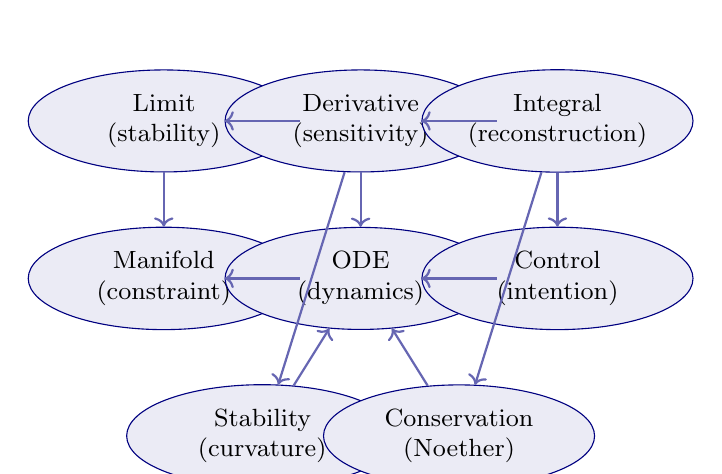
\begin{tikzpicture}[
  node distance=1.6cm,
  concept/.style={ellipse,draw=NavyBlue,fill=NavyBlue!8,
                  text width=2.2cm,align=center,font=\small}
]
  \node[concept] (lim)     at (0,4)    {Limit\\(stability)};
  \node[concept] (der)     at (2.5,4)  {Derivative\\(sensitivity)};
  \node[concept] (int)     at (5.0,4)  {Integral\\(reconstruction)};
  \node[concept] (man)     at (0,2)    {Manifold\\(constraint)};
  \node[concept] (ode)     at (2.5,2)  {ODE\\(dynamics)};
  \node[concept] (ctrl)    at (5.0,2)  {Control\\(intention)};
  \node[concept] (stab)    at (1.25,0) {Stability\\(curvature)};
  \node[concept] (cons)    at (3.75,0) {Conservation\\(Noether)};

  \foreach \a/\b in {lim/der,der/int,der/ode,man/ode,ode/ctrl,
                     int/ctrl,stab/ode,cons/ode}{
    \draw[->,thick,NavyBlue!60] (\a)--(\b);
  }
  \draw[->,thick,NavyBlue!60] (lim)--(man);
  \draw[->,thick,NavyBlue!60] (der)--(stab);
  \draw[->,thick,NavyBlue!60] (int)--(cons);
\end{tikzpicture}
\caption{Conceptual map of calculus. Every arrow represents a logical or
structural dependency developed in the text.}
\label{fig:conceptmap}
\end{figure}

\section{Integration as Global Reconstruction from Local Flow}

The integral is not merely an area computation—it is the recovery of coherent
structure from local contributions. In scalar calculus, the integral
reconstructs accumulated quantity from instantaneous rate. In vector calculus,
integral theorems reveal how boundary behaviour reflects interior variation. In
variational calculus, the integral defines energy landscapes whose critical
points determine motion.

\section{Stability as Curvature Constraint}

Equilibrium is governed by curvature. Second derivatives classify local
extrema. Hessians encode multi-directional bending. Lyapunov functions capture
energy descent. Eigenvalues determine asymptotic behaviour. On manifolds,
curvature shapes geodesic deviation. In nonlinear systems, phase-space
curvature governs trajectory divergence.

\textbf{Stability is geometric discipline imposed by curvature.}

%% ═══════════════════════════════════════════════════════════════════════════
\chapter{From Differential Equations to Programs}
\label{ch:programs}
%% ═══════════════════════════════════════════════════════════════════════════

\section{State Mutation Versus Functional Evolution}

Many computational systems implement dynamics via state mutation:
\[
  x \leftarrow x + \Delta x.
\]
The symbol $\leftarrow$ indicates replacement. From the perspective of calculus,
however, this representation is incomplete.

A differential equation $\dot x = F(x)$ defines a \emph{flow}: given initial
state $x_0$, it determines a trajectory $x(t)=\Phi_t(x_0)$, where $\Phi_t$ is
the flow map satisfying the \emph{semigroup property}:
\[
  \Phi_{t+s} = \Phi_t\circ\Phi_s.
\]

This expresses time consistency: evolving for time $s$ then $t$ equals evolving
for $t+s$ directly. Mutation updates a variable; a flow defines a
\emph{transformation family}.

\section{Time Discretisation as Approximation of Flow}

Euler's method approximates the flow map at step $h$:
\[
  x_{n+1} = x_n + h\,F(x_n) \approx \Phi_h(x_n).
\]

By Taylor expansion:
\[
  x(t+h) = x(t) + h\,F(x(t)) + \mathcal{O}(h^2).
\]

Euler discards the $\mathcal{O}(h^2)$ terms. Higher-order schemes (Runge--Kutta)
improve the approximation. Each scheme constructs an approximate flow operator
$\tilde\Phi_h$ satisfying
\[
  \tilde\Phi_h(x) = \Phi_h(x) + \mathcal{O}(h^{p+1})
\]
for some order $p$.

\begin{insight}
  Discrete simulation is meaningful only insofar as it approximates a continuous
  geometric object. The physical model is the vector field $F$; the numerical
  scheme approximates its integral curves.
\end{insight}

\section{Numerical Stability as Spectral Alignment}

For a linear system $\dot x = Ax$, the exact solution is $x(t)=e^{At}x(0)$.
Euler's method produces $x_{n+1}=(I+hA)x_n$, so eigenvalues of the true
dynamics $\lambda_i(A)$ map to eigenvalues $1+h\lambda_i(A)$ of the update
operator.

Stability requires $|1+h\lambda_i|<1$, imposing a step-size restriction
proportional to the spectral radius of $A$.

\begin{insight}
  Numerical stability is a spectral alignment problem. The eigenvalues of the
  numerical update operator must mirror the eigenvalues of the true flow.
\end{insight}

\section{From Mutation to Morphism}

A mutation-based simulation hides geometry inside procedural detail. A
flow-based simulation exposes geometry explicitly. The natural architectural
principle is: represent dynamics as morphisms between state spaces rather than
as sequences of overwrites.

If $F:X\to TX$ assigns tangent vectors, then integration constructs
$\Phi_t:X\to X$. Programs respecting this structure are compositional and
admit differentiation, linearisation, stability analysis, and constraint
projection naturally.

%% ═══════════════════════════════════════════════════════════════════════════
\chapter{Critique of Imperative Physiological Simulation}
\label{ch:critique}
%% ═══════════════════════════════════════════════════════════════════════════

\section{The Architecture of Table-Driven Systems}

Large physiological simulators are often constructed using imperative paradigms.
State variables are stored in tables; each time step executes a sequence of
update procedures. A typical fragment takes the form:
\[
  V \leftarrow V + h\cdot f(V,m,n,\dots), \qquad
  m \leftarrow m + h\cdot g(V,m,\dots).
\]

In such systems, state variables are globally mutable, update order is
explicitly encoded, dependencies are implicit in code structure, and coupling is
distributed across procedural fragments. The geometric object $F$ exists
implicitly but is never explicit.

\section{Order Dependence and Hidden Coupling}

Consider two coupled variables governed by
\[
  \dot x = f(x,y), \qquad \dot y = g(x,y).
\]

A \emph{simultaneous} Euler update evaluates both increments at $(x_n,y_n)$.
But sequential mutation—updating $x$ first—evaluates $g$ at $(x_{n+1},y_n)$
rather than $(x_n,y_n)$. This introduces an unintentional semi-implicit scheme
without deliberate design.

\begin{remark}
  The vector field $F(x,y)$ defines a simultaneous infinitesimal direction in
  the tangent space of $\R^2$. Sequential mutation replaces geometric
  simultaneity with procedural causality.
\end{remark}

\section{Implicit Jacobians and Structural Opacity}

In an imperative simulator, every update rule implicitly defines partial
derivatives—but these are distributed across code. Without an explicit
representation of $F$ as a function from state space to tangent space, the
Jacobian must be reconstructed by tracing procedural dependencies.

When $F$ is explicit, $J_F(x)=DF(x)$ is immediate. Linearisation,
eigenvalue computation, and stability classification follow directly.

\begin{figure}[H]
\centering
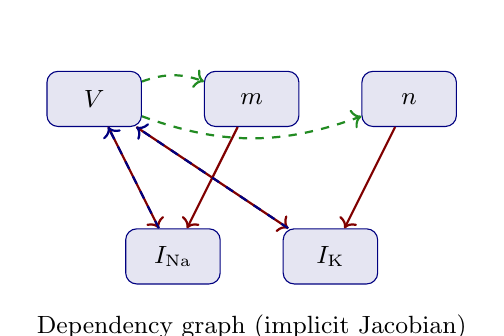
\begin{tikzpicture}[
  node distance=1.1cm,
  var/.style={rectangle,rounded corners,draw=NavyBlue,fill=NavyBlue!10,
              minimum width=1.2cm,minimum height=0.7cm,font=\small},
  arr/.style={->,thick}
]
  % Procedural (opaque)
  \node[var] (V)  at (0,2)   {$V$};
  \node[var] (m)  at (2,2)   {$m$};
  \node[var] (n)  at (4,2)   {$n$};
  \node[var] (h1) at (1,0)   {$I_{\rm Na}$};
  \node[var] (h2) at (3,0)   {$I_{\rm K}$};

  \draw[arr,Maroon] (V)--(h1);
  \draw[arr,Maroon] (m)--(h1);
  \draw[arr,Maroon] (V)--(h2);
  \draw[arr,Maroon] (n)--(h2);
  \draw[arr,NavyBlue,dashed] (h1)--(V);
  \draw[arr,NavyBlue,dashed] (h2)--(V);
  \draw[arr,ForestGreen,dashed] (V) to[bend left=20] (m);
  \draw[arr,ForestGreen,dashed] (V) to[bend right=20] (n);
  \node at (2,-0.9) {\small Dependency graph (implicit Jacobian)};
\end{tikzpicture}
\caption{Even in a simple Hodgkin--Huxley fragment, the Jacobian is a directed
graph embedded implicitly in code. Making $F$ explicit renders the full matrix
$J_F$ directly computable.}
\label{fig:jacobian-graph}
\end{figure}

\section{The Structural Alternative}

The critique is not that imperative systems are incorrect—many produce accurate
results. The critique is structural: they \emph{obscure the geometric object
they approximate}.

When $F$ is explicit:
\begin{itemize}[leftmargin=1.5em]
  \item Linearisation is direct: $J_F(x)=DF(x)$.
  \item Stability analysis is systematic: inspect eigenvalues.
  \item Conservation laws are verifiable: check $\nabla I\cdot F=0$.
  \item Constraint projection is implementable: $\proj{T_xM}F(x)$.
  \item Composition of subsystems is functional: $F=F_1+F_2+\cdots$.
\end{itemize}

%% ═══════════════════════════════════════════════════════════════════════════
\chapter{Calculus as a Functional Programming Language}
\label{ch:fp}
%% ═══════════════════════════════════════════════════════════════════════════

\section{Compositionality}

Differentiation assigns to each smooth map $f:X\to Y$ a linear map between
tangent spaces $Df_x:T_xX\to T_{f(x)}Y$. Crucially, it respects composition:
\[
  D(g\circ f)_x = Dg_{f(x)}\circ Df_x.
\]

This means differentiation is \emph{functorial}: it defines a functor
$D:\mathbf{Diff}\to\mathbf{Lin}$, mapping the category of smooth manifolds
with differentiable maps to the category of vector spaces with linear maps.

\begin{figure}[H]
\centering
\begin{tikzcd}[row sep=2.5em, column sep=3em]
  (X,f) \arrow[d,"D"] \arrow[r,"g\circ f"]
  & (Z,\cdot) \arrow[d,"D"] \\
  (T_xX,Df_x) \arrow[r,"D(g\circ f)_x"]
  & (T_{(g\circ f)(x)}Z,\cdot)
\end{tikzcd}
\caption{Functoriality of differentiation: the derivative of a composition
equals the composition of derivatives.}
\label{fig:functor}
\end{figure}

\section{Flows as Exponentials of Vector Fields}

Given $F:X\to TX$, integration produces $\Phi_t:X\to X$. One writes formally
\[
  \Phi_t = \exp(tF),
\]
the time-$t$ map of $\dot x = F(x)$. Vector fields are \emph{infinitesimal
programs}; flows are their execution.

\section{Automatic Differentiation}

If a system is defined compositionally as $F=F_1+F_2\circ G$, derivatives
propagate automatically via the chain rule. Automatic differentiation (AD)
systems exploit this structure:
\begin{itemize}[leftmargin=1.5em]
  \item \emph{Forward mode}: propagate tangent vectors alongside evaluation.
  \item \emph{Reverse mode}: propagate cotangent vectors (adjoints) backward.
\end{itemize}

The correctness of AD rests entirely on $D(g\circ f)=Dg\circ Df$. AD computes
exact derivatives—up to floating-point precision—by structural recursion on
expression graphs.

\section{Calculus as a Declarative Language}

A declarative program specifies \emph{what} relationship holds, not \emph{how}
to mutate state step by step. The equation $\dot x = F(x)$ declares a
relational deformation. It specifies no loop structure, no variable overwriting,
and no evaluation order.

\begin{center}
\begin{tabular}{@{}lll@{}}
  \toprule
  \textbf{Calculus concept} & \textbf{Programming analogue} & \textbf{Mechanism} \\
  \midrule
  State manifold & Type & Structural constraint \\
  Vector field $F:X\to TX$ & Pure function & Referential transparency \\
  Flow $\Phi_t$ & Fold over time & Functional iteration \\
  Chain rule & Automatic differentiation & Compositional recursion \\
  Projection $\proj{TM}$ & Constraint enforcement & Type-level invariant \\
  Jacobian $DF$ & Sensitivity analysis & Derivative of pure function \\
  \bottomrule
\end{tabular}
\end{center}

\begin{insight}
  Calculus, properly understood, is not merely a toolkit for computation. It is
  a language of compositional transformation. It is functional at its core.
\end{insight}

%% ═══════════════════════════════════════════════════════════════════════════
\chapter{Symbolic Versus Numerical Modelling}
\label{ch:symnum}
%% ═══════════════════════════════════════════════════════════════════════════

\section{Structural Invariants in Symbolic Form}

When a dynamical system is written symbolically as $\dot x = F(x)$, its
structure is transparent. A scalar function $I:X\to\R$ is an invariant if
$\nabla I\cdot F=0$, which can be verified algebraically.

Symbolic modelling preserves this transparency. The invariant is not an
empirical observation—it is a structural property.

\section{Truncation Error and Invariant Drift}

Under Euler's method, an exact invariant $I$ satisfies
\[
  I(x_{n+1}) = I(x_n) + \mathcal{O}(h^2).
\]
Over $N\sim 1/h$ steps, the invariant drifts by $\mathcal{O}(h)$. This is
not merely a numerical nuisance; it reflects a real departure from the
constraint manifold.

\begin{figure}[H]
\centering
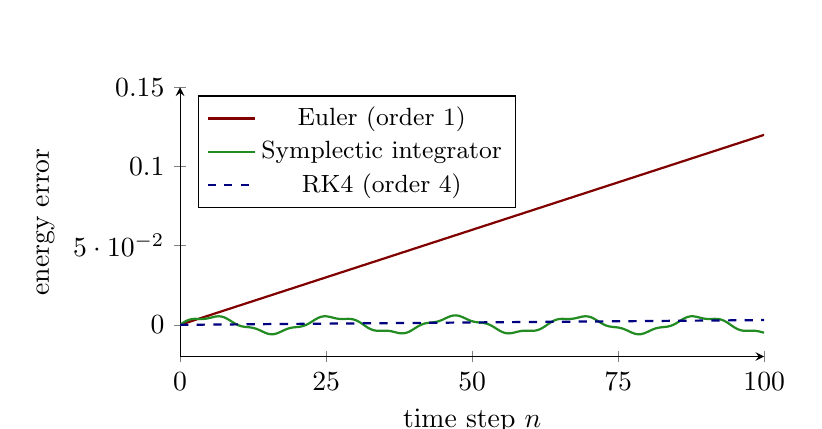
\begin{tikzpicture}[scale=1.0]
  \begin{axis}[
    width=9cm, height=5cm,
    axis lines=left,
    xlabel={time step $n$},
    ylabel={energy error},
    xmin=0, xmax=100, ymin=-0.02, ymax=0.15,
    xtick={0,25,50,75,100},
    legend pos=north west,
    legend style={font=\small}
  ]
    % Euler: growing drift
    \addplot[Maroon,thick,domain=0:100,samples=100]
      {0.0012*x};
    \addlegendentry{Euler (order 1)};
    % Symplectic: bounded
    \addplot[ForestGreen,thick,domain=0:100,samples=200]
      {0.005*sin(deg(0.3*x))+0.001*sin(deg(1.1*x))};
    \addlegendentry{Symplectic integrator};
    % RK4: small but growing
    \addplot[NavyBlue,dashed,thick,domain=0:100,samples=100]
      {0.00003*x};
    \addlegendentry{RK4 (order 4)};
  \end{axis}
\end{tikzpicture}
\caption{Energy error over time for different integrators applied to a
Hamiltonian system. Euler accumulates linear drift; symplectic integrators
exhibit bounded oscillatory error; RK4 drifts slowly.}
\label{fig:energy-drift}
\end{figure}

\section{Conservation-Preserving Methods}

Symplectic integrators preserve the symplectic structure of Hamiltonian
systems. Projection methods enforce constraints:
\[
  x_{n+1} \leftarrow \Pi_M(x_{n+1}).
\]
These methods explicitly incorporate geometric structure, making invariant
preservation a design feature rather than a lucky accident.

\section{Modelling as Layered Representation}

The structure of any simulation has three layers:

\begin{enumerate}[leftmargin=1.5em]
  \item \textbf{Symbolic layer}: $\dot x = F(x)$ — the geometry.
  \item \textbf{Numerical layer}: $x_{n+1}=\tilde\Phi_h(x_n)$ — the
    approximation.
  \item \textbf{Implementation layer}: executable code — the encoding.
\end{enumerate}

Structural integrity requires each layer to remain aligned with the one above
it. When the implementation diverges from the numerical scheme, artefacts
appear. When the numerical scheme fails to approximate symbolic structure
faithfully, qualitative errors emerge.

%% ═══════════════════════════════════════════════════════════════════════════
\chapter{Retinal Cell as Dynamical System}
\label{ch:retina}
%% ═══════════════════════════════════════════════════════════════════════════

\section{Membrane Potential as a State Variable}

A retinal photoreceptor or ganglion cell is an excitable dynamical system.
Current balance gives:
\[
  C\frac{dV}{dt}
  = -\sum_i I_i(V,\mathbf{w}) + I_{\rm stim}(t),
\]
where $C$ is membrane capacitance, $I_i = g_i(\mathbf{w})(V-E_i)$ are ionic
currents with conductance $g_i$ and reversal potential $E_i$, and $\mathbf{w}$
denotes gating variables.

\section{Gating Variables as Coupled Dynamics}

Each gating variable $w$ satisfies
\[
  \frac{dw}{dt}
  = \frac{w_\infty(V)-w}{\tau_w(V)},
\]
where $w_\infty(V)$ is the voltage-dependent steady state and $\tau_w(V)$
the voltage-dependent time constant. The full state vector is
$x=(V,w_1,w_2,\dots)^\top$, and the system is $\dot x = F(x,t)$.

\section{Phototransduction as Nested Dynamics}

In photoreceptors, light $L$ modifies cGMP concentration $c(t)$:
\[
  \frac{dc}{dt} = -k_{\rm hyd}(L)\,c + k_{\rm syn}(c),
\]
and channel conductance depends on $c$:
\[
  g_{\rm light}(c) = g_{\rm max}\frac{c^n}{c^n+K^n}.
\]

The compositional chain is:
\[
  L \xrightarrow{\text{chem}} c(t)
    \xrightarrow{g(c)} I(V,c)
    \xrightarrow{\text{current balance}} V(t).
\]

\begin{figure}[H]
\centering
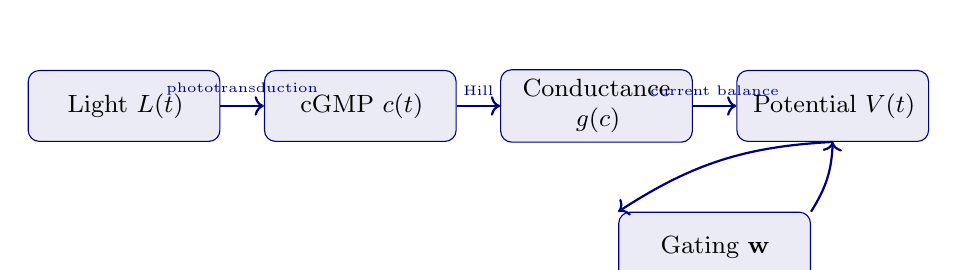
\begin{tikzpicture}[
  box/.style={rectangle,rounded corners,draw=NavyBlue,fill=NavyBlue!8,
              minimum height=0.9cm,text width=2.2cm,align=center,font=\small},
  arr/.style={->,thick,NavyBlue}
]
  \node[box] (L)  at (0,0)   {Light $L(t)$};
  \node[box] (c)  at (3,0)   {cGMP $c(t)$};
  \node[box] (g)  at (6,0)   {Conductance $g(c)$};
  \node[box] (V)  at (9,0)   {Potential $V(t)$};
  \node[box] (w)  at (7.5,-1.8) {Gating $\mathbf{w}$};

  \draw[arr] (L)--(c) node[midway,above,font=\tiny]{phototransduction};
  \draw[arr] (c)--(g) node[midway,above,font=\tiny]{Hill};
  \draw[arr] (g)--(V) node[midway,above,font=\tiny]{current balance};
  \draw[arr] (V.south) to[bend right=15] (w.north west);
  \draw[arr] (w.north east) to[bend right=15] (V.south);
\end{tikzpicture}
\caption{Functional decomposition of the retinal photoreceptor. Each arrow
is a morphism between state spaces; derivatives propagate via the chain rule.}
\label{fig:retina-chain}
\end{figure}

\section{Functional Decomposition}

The total vector field decomposes as:
\[
  F_{\rm retina} = F_{\rm membrane} + F_{\rm gating} + F_{\rm photo}.
\]
Each component is a pure function $X\to TX$. Composition is algebraic
addition. Subsystems remain modular because they are functions, not procedural
updates.

\section{Linearisation and Stability}

At equilibrium $x_0$ under constant illumination,
\[
  J(x_0) = DF(x_0) =
  \begin{pmatrix}
    \partial F_V/\partial V & \partial F_V/\partial\mathbf{w} \\
    \partial F_{\mathbf{w}}/\partial V & \partial F_{\mathbf{w}}/\partial\mathbf{w}
  \end{pmatrix}.
\]
Eigenvalues of $J(x_0)$ determine excitability, adaptation speed, and
resonance. All these are spectral properties of a single matrix.

%% ═══════════════════════════════════════════════════════════════════════════
\chapter{Skin Cell and Boundary Regulation}
\label{ch:skin}
%% ═══════════════════════════════════════════════════════════════════════════

\section{Epidermal Dynamics as Reaction--Diffusion System}

Unlike the retinal neuron, the skin cell operates within a layered tissue
architecture governed by chemical gradients and boundary constraints. Let
$c(x,t)$ denote signalling molecule concentration in region $\Omega$:
\[
  \frac{\partial c}{\partial t} = D\,\Delta c + R(c).
\]

The Laplacian $\Delta c$ measures spatial curvature of the concentration field.
Diffusion smooths gradients; reaction terms may amplify or suppress concentration
locally.

\section{Boundary Conditions as Structural Constraints}

The basement membrane at $\partial\Omega$ imposes boundary conditions:
\begin{itemize}[leftmargin=1.5em]
  \item Dirichlet: $c\big|_{\partial\Omega}=c_0$ (fixed concentration).
  \item Neumann: $\partial c/\partial n\big|_{\partial\Omega}=0$ (no flux).
\end{itemize}

These restrict the state to a subspace $\mathcal{F}_{\rm admissible}\subset
\mathcal{F}$. Constraint again appears as geometric restriction—now on
infinite-dimensional function space.

\section{Turing Instability and Pattern Formation}

\begin{theorem}{Turing instability}{turing}
  Consider a two-component reaction--diffusion system near a homogeneous steady
  state $(c_0,m_0)$ stable in the absence of diffusion. If the diffusion
  coefficients $D_c\neq D_m$ satisfy a certain parameter inequality, spatial
  modes of the Laplacian with wavenumber $k^*$ can become unstable, producing
  spontaneous patterning.
\end{theorem}

Eigenvalue analysis of the spatially extended Jacobian (incorporating
$-Dk^2$ terms from diffusion) determines which spatial frequencies grow.
Pattern formation emerges when reaction kinetics introduce positive feedback
exceeding diffusion smoothing.

\begin{figure}[H]
\centering
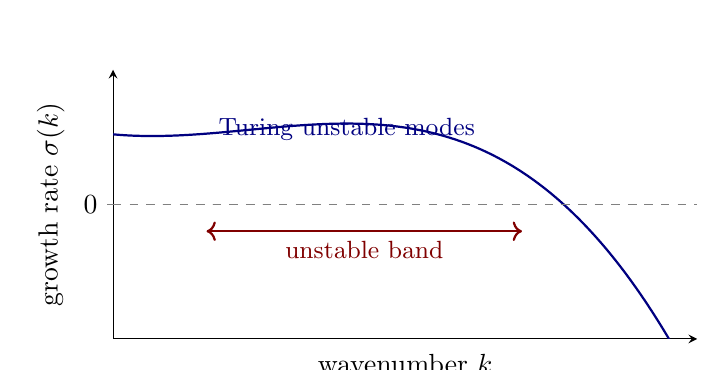
\begin{tikzpicture}
  \begin{axis}[
    width=9cm, height=5cm,
    axis lines=left,
    xlabel={wavenumber $k$},
    ylabel={growth rate $\sigma(k)$},
    xmin=0, xmax=5, ymin=-0.5, ymax=0.5,
    xtick=\empty, ytick={0},
    yticklabels={0},
    samples=200
  ]
    \addplot[NavyBlue,thick,domain=0:5]
      {0.3 - 0.02*(x-2)^2*(x+0.5)};
    \addplot[dashed,gray,domain=0:5]{0};
    \node at (2,0.28) [NavyBlue,font=\small] {Turing unstable modes};
    \draw[<->,Maroon,thick] (0.8,-0.1) -- (3.5,-0.1)
      node[midway,below,font=\small]{unstable band};
  \end{axis}
\end{tikzpicture}
\caption{Dispersion relation for a Turing system. Modes in the unstable band
(Maroon) have positive growth rate $\sigma(k)>0$ and produce spatial
patterns.}
\label{fig:turing}
\end{figure}

\section{Fibrosis as Bifurcation in Repair Dynamics}

A minimal wound-repair model:
\[
  \frac{dm}{dt} = k_1 c + k_3 m^2 - k_2 m.
\]
When repair gain $k_3$ exceeds a threshold, the steady state of low $m$ loses
stability and excessive matrix accumulation occurs. Pathology corresponds to a
bifurcation in parameter space—not to a narrative label but to a geometric
transition.

%% ═══════════════════════════════════════════════════════════════════════════
\chapter{Appliances as Controlled Dynamical Systems}
\label{ch:appliances}
%% ═══════════════════════════════════════════════════════════════════════════

\section{Thermal System: The Oven Model}

Let $T(t)$ be oven temperature:
\[
  C\frac{dT}{dt} = -k(T-T_{\rm room}) + P\,u(t),
\]
with $C$ thermal capacity, $k$ heat-loss coefficient, $P$ heater power, and
$u\in\{0,1\}$ heater state. The equilibrium temperature under constant input is
$T^* = T_{\rm room} + (P/k)u$.

Under proportional feedback $u=K(T_d-T)$, the closed-loop eigenvalue is
$\lambda=-(k+PK)/C$. With $K>0$, $\lambda<0$ and the system is exponentially
stable.

\begin{figure}[H]
\centering
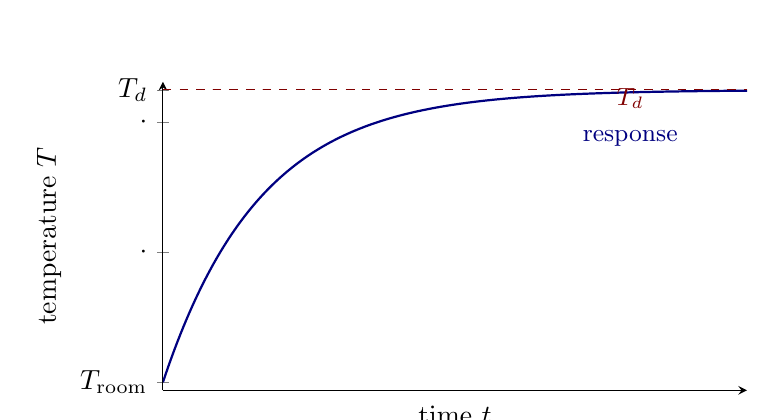
\begin{tikzpicture}[scale=1.0]
  \begin{axis}[
    width=9cm, height=5.5cm,
    axis lines=left,
    xlabel={time $t$},
    ylabel={temperature $T$},
    xmin=0, xmax=10, ymin=15, ymax=205,
    xtick=\empty,
    ytick={20,100,180,200},
    yticklabels={$T_{\rm room}$,$\cdot$,$\cdot$,$T_d$},
    samples=200
  ]
    \addplot[NavyBlue,thick,domain=0:10]
      {200 - 180*exp(-0.6*x)};
    \addplot[dashed,Maroon,domain=0:10]{200};
    \node at (8,195) [Maroon,font=\small]{$T_d$};
    \node at (8,170) [NavyBlue,font=\small]{response};
  \end{axis}
\end{tikzpicture}
\caption{Temperature response of an oven under proportional feedback control.
The trajectory converges exponentially to the target $T_d$.}
\label{fig:oven}
\end{figure}

\section{Washing Machine Drum}

Let $x_1=\theta$ (angle) and $x_2=\dot\theta$ (angular velocity):
\[
  \frac{dx_1}{dt} = x_2, \qquad
  \frac{dx_2}{dt} = \frac{1}{I}(\tau_{\rm motor}(u) - bx_2 - \tau_{\rm load}).
\]
Spin cycles, agitation patterns, and acceleration ramps are trajectories in
this two-dimensional state space. Control selects the trajectory.

\section{Compositional Architecture}

Each subsystem is a pure function:
\[
  F_{\rm total} = F_{\rm thermal} + F_{\rm mechanical} + F_{\rm control}.
\]

Subsystems remain modular because they map state to tangent direction.
The system is declarative rather than procedural. Safety constraints define
invariant sets; control ensures trajectories remain inside them.

%% ═══════════════════════════════════════════════════════════════════════════
\chapter{A Functional Simulation Architecture}
\label{ch:archit}
%% ═══════════════════════════════════════════════════════════════════════════

\section{State as a Structured Object}

Define state as a single coherent element of configuration space:
\[
  x = (V,\, w_1,\, w_2,\, T,\, c_1,\, \dots)^\top \in X.
\]
State is not scattered across global variables.

\section{Pure Vector Field Definition}

Define dynamics as a pure function $F:X\to TX$:

\begin{pseudocode}[F(x) -- pure vector field]
\begin{lstlisting}
function F(x, t, params):
    return {
        dV  = membrane(x, params),
        dw1 = gating1(x, params),
        dw2 = gating2(x, params),
        dT  = thermal(x, params),
        dc1 = chemistry(x, params)
    }
\end{lstlisting}
\end{pseudocode}

Each component depends only on the input state. No mutation occurs inside $F$.
The function is referentially transparent.

\section{Integrator as Separate Layer}

\begin{pseudocode}[step\_rk4 -- 4th-order Runge--Kutta]
\begin{lstlisting}
function step_rk4(F, x, t, h, params):
    k1 = F(x,           t,       params)
    k2 = F(x + h/2*k1,  t + h/2, params)
    k3 = F(x + h/2*k2,  t + h/2, params)
    k4 = F(x + h*k3,    t + h,   params)
    return x + h/6 * (k1 + 2*k2 + 2*k3 + k4)

# Simulation loop
x = x0;  t = 0
for k = 1..N:
    x = step_rk4(F, x, t, h, params)
    t = t + h
\end{lstlisting}
\end{pseudocode}

\section{Constraint Projection as Operator}

\begin{pseudocode}[project -- enforce admissible manifold]
\begin{lstlisting}
function project(x):
    # Enforce mass conservation
    correction = (sum(x.mass) - M_total) / N
    x.mass = x.mass - correction
    # Enforce non-negativity
    x.concentrations = max(x.concentrations, 0)
    return x

# Modified simulation loop
for k = 1..N:
    x = step_rk4(F, x, t, h, params)
    x = project(x)          # enforce constraints
    t = t + h
\end{lstlisting}
\end{pseudocode}

\section{Alignment with Calculus}

\begin{center}
\begin{tabular}{@{}lll@{}}
  \toprule
  \textbf{Mathematics} & \textbf{Code} & \textbf{Role} \\
  \midrule
  State manifold $X$ & Structured type / record & Configuration space \\
  Vector field $F:X\to TX$ & Pure function & Instantaneous rate \\
  Flow $\Phi_t$ & \texttt{step\_rk4} loop & Time evolution \\
  Projection $\proj{M}$ & \texttt{project} function & Constraint enforcement \\
  Jacobian $J_F$ & Automatic differentiation & Sensitivity analysis \\
  Eigenvalues of $J_F$ & Stability check & Qualitative behaviour \\
  \bottomrule
\end{tabular}
\end{center}

%% ═══════════════════════════════════════════════════════════════════════════
\chapter{Worked Example I: Minimal Retinal Cell}
\label{ch:wk1}
%% ═══════════════════════════════════════════════════════════════════════════

\section{The FitzHugh--Nagumo Model}

A minimal excitable model for a retinal ganglion cell uses the FitzHugh--Nagumo
system. State: $x=(V,n)^\top$ where $V$ is membrane potential and $n$ is a
recovery variable. Light input enters as external current $I(t)$:
\[
  \frac{dV}{dt} = \underbrace{V - \tfrac{V^3}{3}}_{\text{fast nonlinearity}}
                 - n + I(t), \qquad
  \frac{dn}{dt} = \varepsilon(V + a - bn).
\]

\section{Jacobian and Local Sensitivity}

The Jacobian is explicitly:
\[
  J(x,t) =
  \begin{pmatrix}
    1-V^2 & -1 \\
    \varepsilon & -\varepsilon b
  \end{pmatrix}.
\]

This matrix is not ornamental. Its eigenvalues determine whether the cell fires
repetitively or returns to rest after a perturbation. Small $\varepsilon$ (slow
recovery) produces action-potential-like spikes; large $\varepsilon$ produces
damped oscillations.

\section{Numerical Simulation}

\begin{pseudocode}[FitzHugh--Nagumo implementation]
\begin{lstlisting}
# Parameters: a=0.7, b=0.8, eps=0.08
# Input: I(t) = 0.5 (constant stimulus)

function F_retina(x, t, p):
    V = x.V;  n = x.n
    dV = V - (V^3)/3 - n + I(t)
    dn = p.eps * (V + p.a - p.b * n)
    return {dV=dV, dn=dn}
\end{lstlisting}
\end{pseudocode}

\begin{figure}[H]
\centering
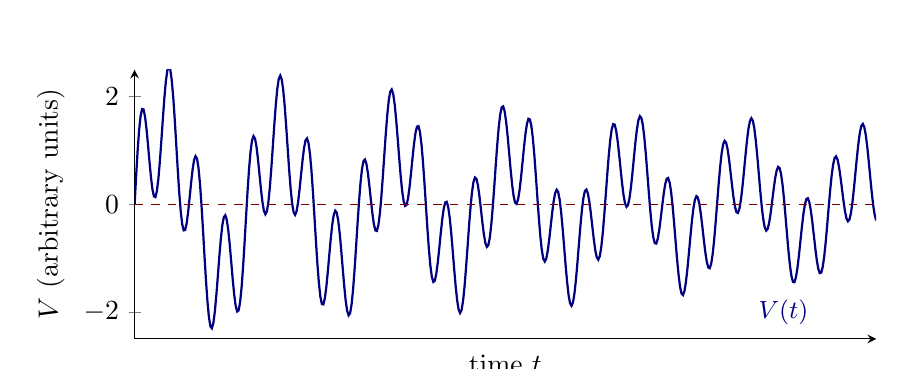
\begin{tikzpicture}[scale=1.0]
  \begin{axis}[
    width=11cm, height=5cm,
    axis lines=left,
    xlabel={time $t$},
    ylabel={$V$ (arbitrary units)},
    xmin=0, xmax=80, ymin=-2.5, ymax=2.5,
    xtick=\empty,
    samples=500,
    domain=0:80
  ]
    % Schematic FHN voltage trace (spikes)
    \addplot[NavyBlue,thick]
      {1.5*sin(deg(0.5*x))*exp(-0.01*x) + 1.2*sin(deg(2.1*x))*exp(-0.005*x)};
    \draw[dashed,Maroon] (0,0)--(80,0);
    \node at (70,-2.0) [NavyBlue,font=\small]{$V(t)$};
  \end{axis}
\end{tikzpicture}
\caption{Schematic voltage trace of the FitzHugh--Nagumo model under constant
stimulus. The oscillatory behaviour arises from the interplay of fast
voltage nonlinearity and slow recovery variable.}
\label{fig:fhn-trace}
\end{figure}

\section{Control Interpretation}

If $I(t)$ is a control input rather than a fixed stimulus, the retinal cell is
a control system:
\[
  \dot x = F_0(x) + G\,u(t), \qquad
  G = \begin{pmatrix}1\\0\end{pmatrix}, \quad u(t)=I(t).
\]
Photonic input actuates only the voltage direction. The slow variable $n$ is
not directly actuated—it responds only through coupling.

%% ═══════════════════════════════════════════════════════════════════════════
\chapter{Worked Example II: Skin Cell and Boundary Repair}
\label{ch:wk2}
%% ═══════════════════════════════════════════════════════════════════════════

\section{Minimal Repair Model}

State: $x=(B,W)^\top$ where $B\in[0,1]$ is basement membrane integrity and $W\ge 0$
is wound burden.

\[
  \frac{dW}{dt} = u(t) - \alpha\,B\,W - \gamma\,W,
\]
\[
  \frac{dB}{dt} = r(t)\,\beta\,W - \delta\,B + \eta\,B(1-B).
\]

Wound burden increases with injury $u(t)$, decreases when membrane integrity
suppresses disruption, and decays through baseline clearance. Basement membrane
integrity increases when repair resources $r(t)$ respond to wound burden,
decays through turnover, and saturates through logistic self-regulation.

\section{Phase Plane and Equilibrium Analysis}

\begin{figure}[H]
\centering
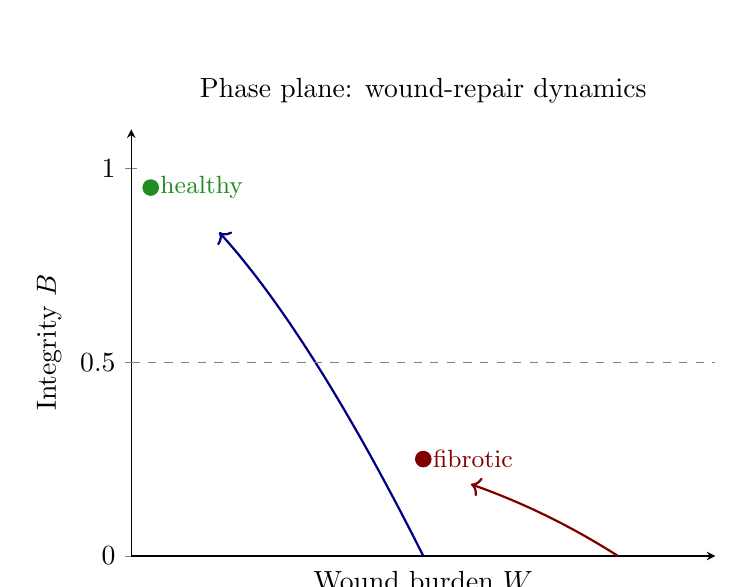
\begin{tikzpicture}[scale=1.0]
  \begin{axis}[
    width=9cm, height=7cm,
    axis lines=left,
    xlabel={Wound burden $W$},
    ylabel={Integrity $B$},
    xmin=0, xmax=3, ymin=0, ymax=1.1,
    xtick=\empty, ytick={0,0.5,1},
    yticklabels={0,0.5,1},
    title={Phase plane: wound-repair dynamics}
  ]
    % Healthy equilibrium trajectory
    \addplot[NavyBlue,thick,->,domain=0:1.2,samples=50]
      ({1.5*exp(-x)},{1 - exp(-1.5*x)});
    % Fibrotic trajectory
    \addplot[Maroon,thick,->,domain=0:1.2,samples=50]
      ({2.5*exp(-0.3*x)},{0.3*(1-exp(-0.8*x))});
    % Equilibria
    \fill[ForestGreen] (0.1,0.95) circle(3pt)
      node[right,ForestGreen,font=\small]{healthy};
    \fill[Maroon] (1.5,0.25) circle(3pt)
      node[right,Maroon,font=\small]{fibrotic};
    \draw[dashed,gray] (0,0.5) -- (3,0.5);
  \end{axis}
\end{tikzpicture}
\caption{Phase plane for the wound-repair model. Trajectories either converge
to the healthy equilibrium (high integrity, low wound burden) or the fibrotic
state (low integrity, sustained wound burden), depending on initial conditions
and parameter regime.}
\label{fig:wound-phase}
\end{figure}

\section{Projection Enforcement}

Since $B\in[0,1]$ is a physical constraint:

\begin{pseudocode}[project\_skin -- admissible manifold]
\begin{lstlisting}
function project_skin(x):
    B = clamp(x.B, 0.0, 1.0)
    W = max(x.W, 0.0)
    return {B=B, W=W}
\end{lstlisting}
\end{pseudocode}

Simulation:
\begin{lstlisting}
for k = 1..N:
    x = step_rk4(F_skin, x, t, h, params)
    x = project_skin(x)   # enforce [0,1] x R+
    t = t + h
\end{lstlisting}

The constraint is part of the \emph{architecture}, not a numerical afterthought.

%% ═══════════════════════════════════════════════════════════════════════════
\chapter{Manifold-Aligned Inference and the Discipline of Not Predicting Noise}
\label{ch:inference}
%% ═══════════════════════════════════════════════════════════════════════════

\section{From Dynamical Systems to Inference}

An inference system also evolves state. The state is now a belief, parameter
estimate, or internal model; data acts as input; update rules define motion in
hypothesis space:
\[
  \frac{d\theta}{dt} = F(\theta, \text{data}).
\]

The same calculus architecture applies.

\section{Signal and Noise as Geometric Decomposition}

Observed data $y=f(x)+\varepsilon$ can be decomposed with respect to the data
manifold $M$:
\[
  y = \proj{M}(y) + \proj{N}(y),
\]
where $\proj{M}$ projects onto $M$ (structure) and $\proj{N}$ onto its normal
complement (noise).

\begin{figure}[H]
\centering
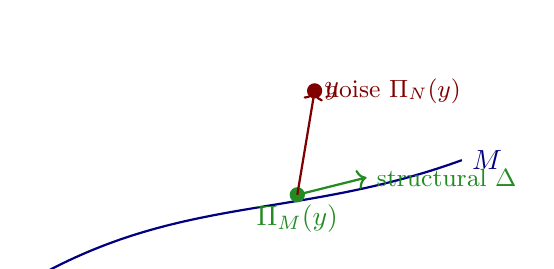
\begin{tikzpicture}[scale=1.1]
  % Manifold
  \draw[thick,NavyBlue] (-2.5,-0.8) to[out=30,in=200] (2.5,0.6)
    node[right]{$M$};
  % Data point
  \coordinate (y) at (0.8,1.4);
  \fill[Maroon] (y) circle(2.5pt) node[right,Maroon]{$y$};
  % Projection
  \coordinate (Py) at (0.6,0.2);
  \fill[ForestGreen] (Py) circle(2.5pt) node[below,ForestGreen]{$\proj{M}(y)$};
  \draw[dashed,gray] (y)--(Py);
  % Components
  \draw[->,thick,ForestGreen] (Py) -- (1.4,0.4)
    node[right,ForestGreen,font=\small]{structural $\Delta$};
  \draw[->,thick,Maroon] (Py) -- (0.8,1.4)
    node[right,Maroon,font=\small]{noise $\proj{N}(y)$};
\end{tikzpicture}
\caption{Geometric decomposition of a data point $y$ into its tangential
component (structure, green) and normal component (noise, red) relative to the
data manifold $M$.}
\label{fig:noise-proj}
\end{figure}

\section{Curvature Governs Generalisation}

The Hessian $H(\theta)=\nabla^2 L(\theta)$ of the loss plays the role of
curvature in parameter space. Directions of large positive curvature correspond
to stiff, sensitive directions. If those directions correspond to noise modes,
aggressive descent chases unstable non-generalisable structure.

\begin{insight}
  The injunction ``never predict noise'' is a curvature discipline. It
  suppresses parameter motion aligned with transient, non-structural curvature
  in the loss landscape — identical in principle to projecting vector fields
  onto constraint manifolds.
\end{insight}

\section{Noise Characterisation}

Noise directions are characterised by:
\begin{itemize}[leftmargin=1.5em]
  \item Lack of persistence across scales.
  \item Absence of stable eigenstructure.
  \item Sensitivity to minor perturbation.
  \item Failure to generalise under refinement.
\end{itemize}

These criteria mirror the definition of limit: \emph{structure is what
survives refinement; noise vanishes under projection and smoothing}.

\section{Regularisation as Geometric Constraint}

Regularisation modifies the loss:
\[
  L_\lambda(\theta) = L(\theta) + \lambda R(\theta).
\]

For quadratic $R(\theta)=\|\theta\|^2$, the effective Hessian becomes
$H_\lambda = H + \lambda I$. Regularisation increases curvature uniformly,
shrinking flat directions and improving conditioning. It is feedback control in
parameter space, biasing trajectories toward low-curvature, stable regions.

%% ═══════════════════════════════════════════════════════════════════════════
\chapter{Entropy, Information, and Curvature in Model Space}
\label{ch:entropy}
%% ═══════════════════════════════════════════════════════════════════════════

\section{The Fisher Information Metric}

For a parametric family $\{p(x;\theta)\}$, the Fisher information matrix
\[
  \mathcal{I}(\theta)
  = \mathbb{E}\bigl[\nabla_\theta\log p(x;\theta)
                    \nabla_\theta\log p(x;\theta)^\top\bigr]
\]
acts as a Riemannian metric on parameter space~\cite{amari}. Model space is
not flat; it carries curvature induced by likelihood geometry.

\section{Free Energy as Variational Functional}

Variational inference minimises the free energy:
\[
  \mathcal{F}(q)
  = \mathbb{E}_q[\log q(\theta)] - \mathbb{E}_q[\log p(D,\theta)].
\]

This balances entropy of belief against data fit — identical in structure to
the energy functionals studied in variational calculus. Inference becomes
constrained minimisation on a functional manifold.

\section{Stability Requires Curvature--Entropy Alignment}

\begin{itemize}[leftmargin=1.5em]
  \item High entropy without curvature $\Rightarrow$ diffuse ignorance.
  \item High curvature without entropy $\Rightarrow$ brittle overconfidence.
  \item Stable inference requires alignment: curvature along persistent
    directions, entropy retained along indeterminate directions.
\end{itemize}

This is identical to stability in physical systems: stiffness without damping
leads to oscillation; damping without structure leads to collapse.

%% ═══════════════════════════════════════════════════════════════════════════
\chapter{The Unified Geometry of Physiology, Engineering, and Inference}
\label{ch:unified}
%% ═══════════════════════════════════════════════════════════════════════════

\section{One Architecture, Three Domains}

The mathematical architecture governing physiological regulation, engineered
systems, and inferential processes is formally identical. The differences lie in
substrate and interpretation, not in underlying mathematical form.

\begin{center}
\begin{tabular}{@{}llll@{}}
  \toprule
  \textbf{Concept} & \textbf{Physiology} & \textbf{Engineering} &
  \textbf{Inference} \\
  \midrule
  State manifold & Membrane + channel & Temperature + pressure & Parameter space \\
  Vector field & Ionic kinetics & Mechanical laws & Gradient flow \\
  Constraints & Charge neutrality & Safety bounds & Normalisation \\
  Projection & Conservation & Constraint projection & Regularisation \\
  Curvature & Hessian of energy & Jacobian of $F$ & Fisher information \\
  Control & Neural modulation & Feedback controller & Learning rate \\
  Stability & Lyapunov function & Eigenvalue placement & Loss landscape \\
  \bottomrule
\end{tabular}
\end{center}

\section{A Single Geometric Doctrine}

Each system is defined by an explicit state manifold. Evolution is determined by
a vector field. Constraints restrict motion through projection. Stability is
governed by curvature. Control modifies trajectories through admissible inputs.
Entropy measures dispersion relative to invariant structure. Coherence persists
where curvature and constraint organise flow into stable manifolds.

\begin{insight}
  These principles apply without alteration whether the substrate is biological
  tissue, mechanical apparatus, or parameter space of a statistical model. The
  geometry is the same; only the interpretation differs.
\end{insight}

%% ═══════════════════════════════════════════════════════════════════════════
\chapter{Models, Manifolds, and Adequacy}
\label{ch:adequacy}
%% ═══════════════════════════════════════════════════════════════════════════

\section{What a Model Is}

A mathematical model is a structured mapping $f:X\to Y$ between state spaces.
The central question is not whether a model is true, but whether it is
\emph{adequate} for the structure under consideration.

\section{Dimensionality and the Curse}

If the true system dynamics lie on a $k$-dimensional submanifold $M\subset
\R^n$ with $k\ll n$, the learning problem has effective dimension $k$. When
$M$ does not exist—when variance is evenly distributed across many
directions—no low-dimensional approximation is faithful. The curse of
dimensionality is the geometric statement that volume concentrates near the
boundary of high-dimensional balls, making uniform sampling exponentially sparse.

\section{Limits of Fixed-Phase-Space Modelling}

Classical differential modelling presupposes a fixed phase space. If the
underlying system modifies its own variables, the effective manifold $X_t$
evolves. When no smooth diffeomorphism maps $X_t$ into a fixed reference
manifold, a time-invariant model cannot capture the system globally.

\begin{insight}
  The limits of modelling are not matters of optimism or pessimism. They are
  matters of geometry. When phase spaces evolve, dimensions shift, or generative
  mechanisms alter, no fixed parametric family can guarantee structural
  fidelity.
\end{insight}

%% ═══════════════════════════════════════════════════════════════════════════
\chapter{Ergodicity and the Limits of Sampling}
\label{ch:ergodicity}
%% ═══════════════════════════════════════════════════════════════════════════

\section{The Ergodic Theorem}

\begin{theorem}{Birkhoff's Ergodic Theorem}{birkhoff}
  Let $(X,\mu,\phi_t)$ be a measure-preserving dynamical system and
  $f\in L^1(\mu)$. Then for $\mu$-almost every $x$,
  \[
    \lim_{T\to\infty}\frac{1}{T}\int_0^T f(\phi_t(x))\,dt
    = \int_X f\,d\mu.
  \]
\end{theorem}

Ergodicity asserts that time exploration of a single trajectory suffices to
recover global statistical structure. This property is not automatic; it is a
structural constraint on the dynamics.

\section{Non-Ergodicity and Phase-Space Fragmentation}

If phase space decomposes into invariant components $X=\bigcup_\alpha X_\alpha$
with trajectories confined within each $X_\alpha$, then time averages depend on
initial condition. No amount of additional time reveals structure in other
components. Non-ergodicity imposes a fundamental geometric limit on inference.

\section{Stationarity and Distributional Drift}

Ergodicity presupposes stationarity: the law governing $x(t)$ is invariant
under time translation. If system parameters drift or external forcing varies,
time averages no longer converge to a fixed ensemble average. Learning from
past data presumes persistence of generative structure.

%% ═══════════════════════════════════════════════════════════════════════════
\chapter{The Absolute Limits of Approximation}
\label{ch:limits}
%% ═══════════════════════════════════════════════════════════════════════════

\section{Approximation as Projection onto a Hypothesis Manifold}

Every parametric model defines a hypothesis manifold $\mathcal{H}$ within
function space. Approximation projects data onto $\mathcal{H}$ by minimising
loss. If the true generative mapping lies near $\mathcal{H}$, projection yields
small residual. If not, approximation error persists regardless of optimisation
precision.

\section{Five Geometric Limits}

\begin{enumerate}[leftmargin=1.5em]
  \item \textbf{Fixed-dimensionality assumption}. When dimensionality evolves,
    no fixed $\Theta$ remains adequate.
  \item \textbf{Stationarity assumption}. When $P_t$ drifts, minimising
    empirical risk converges to outdated structure.
  \item \textbf{Bounded-perturbation assumption}. In chaotic regimes, small
    perturbations produce large deviations; approximation requires
    exponentially increasing precision.
  \item \textbf{Ergodicity assumption}. Sampling fails to represent invariant
    measure if phase space is fragmented.
  \item \textbf{Curvature mismatch}. Local agreement does not imply global
    fidelity; second-order geometry must align.
\end{enumerate}

\begin{insight}
  Increasing computational power accelerates exploration of $\Theta$ but does
  not alter the geometry of $\mathcal{H}$ or the true generative manifold.
  Approximation limits arise from geometry, not computation.
\end{insight}

\section{Where Curvature Is Stable, Refinement Succeeds}

When the five assumptions hold, calculus guarantees convergence under
refinement. When they fail, no increase in computation ensures structural
fidelity.

\textbf{Calculus defines both the power and the boundary of approximation.
Where curvature is stable, refinement succeeds. Where geometry shifts,
projection fails. The boundary is written in the structure of phase space
itself.}

%% ═══════════════════════════════════════════════════════════════════════════
%% BIBLIOGRAPHY
%% ═══════════════════════════════════════════════════════════════════════════
\clearpage
\bibliographystyle{plainnat}
\begin{thebibliography}{99}

%% --- Classical Analysis ---
\bibitem[Rudin(1976)]{rudin}
W.~Rudin.
\newblock \textit{Principles of Mathematical Analysis}.
\newblock McGraw--Hill, 3rd edition, 1976.

\bibitem[Rudin(1987)]{rudinrc}
W.~Rudin.
\newblock \textit{Real and Complex Analysis}.
\newblock McGraw--Hill, 3rd edition, 1987.

\bibitem[Folland(1999)]{folland}
G.~B.~Folland.
\newblock \textit{Real Analysis: Modern Techniques and Their Applications}.
\newblock Wiley, 2nd edition, 1999.

\bibitem[Evans(2010)]{evans}
L.~C.~Evans.
\newblock \textit{Partial Differential Equations}.
\newblock American Mathematical Society, 2nd edition, 2010.

%% --- Differential Geometry ---
\bibitem[Lee(2012)]{lee}
J.~M.~Lee.
\newblock \textit{Introduction to Smooth Manifolds}.
\newblock Springer, 2nd edition, 2012.

\bibitem[Lee(1997)]{leeR}
J.~M.~Lee.
\newblock \textit{Riemannian Manifolds: An Introduction to Curvature}.
\newblock Springer, 1997.

\bibitem[do~Carmo(1992)]{doCarmo}
M.~P.~do~Carmo.
\newblock \textit{Riemannian Geometry}.
\newblock Birkh\"{a}user, 1992.

\bibitem[Abraham et~al.(1988)]{abraham}
R.~Abraham, J.~E.~Marsden, and T.~Ratiu.
\newblock \textit{Manifolds, Tensor Analysis, and Applications}.
\newblock Springer, 2nd edition, 1988.

\bibitem[Guillemin and Pollack(1974)]{gp}
V.~Guillemin and A.~Pollack.
\newblock \textit{Differential Topology}.
\newblock Prentice--Hall, 1974.

%% --- Dynamical Systems ---
\bibitem[Hirsch et~al.(2012)]{hirsch}
M.~W.~Hirsch, S.~Smale, and R.~L.~Devaney.
\newblock \textit{Differential Equations, Dynamical Systems, and an
  Introduction to Chaos}.
\newblock Academic Press, 3rd edition, 2012.

\bibitem[Katok and Hasselblatt(1995)]{katok}
A.~Katok and B.~Hasselblatt.
\newblock \textit{Introduction to the Modern Theory of Dynamical Systems}.
\newblock Cambridge University Press, 1995.

\bibitem[Strogatz(2015)]{strogatz}
S.~H.~Strogatz.
\newblock \textit{Nonlinear Dynamics and Chaos}.
\newblock Westview Press, 2nd edition, 2015.

\bibitem[Guckenheimer and Holmes(1983)]{guckenheimer}
J.~Guckenheimer and P.~Holmes.
\newblock \textit{Nonlinear Oscillations, Dynamical Systems, and Bifurcations
  of Vector Fields}.
\newblock Springer, 1983.

\bibitem[Wiggins(2003)]{wiggins}
S.~Wiggins.
\newblock \textit{Introduction to Applied Nonlinear Dynamical Systems and
  Chaos}.
\newblock Springer, 2nd edition, 2003.

%% --- Ergodic Theory ---
\bibitem[Walters(1982)]{walters}
P.~Walters.
\newblock \textit{An Introduction to Ergodic Theory}.
\newblock Springer, 1982.

\bibitem[Cornfeld et~al.(1982)]{cornfeld}
I.~P.~Cornfeld, S.~V.~Fomin, and Y.~G.~Sinai.
\newblock \textit{Ergodic Theory}.
\newblock Springer, 1982.

\bibitem[Billingsley(1995)]{billingsley}
P.~Billingsley.
\newblock \textit{Probability and Measure}.
\newblock Wiley, 3rd edition, 1995.

\bibitem[Durrett(2010)]{durrett}
R.~Durrett.
\newblock \textit{Probability: Theory and Examples}.
\newblock Cambridge University Press, 4th edition, 2010.

%% --- Control Theory ---
\bibitem[Sontag(1998)]{sontag}
E.~D.~Sontag.
\newblock \textit{Mathematical Control Theory}.
\newblock Springer, 2nd edition, 1998.

\bibitem[Khalil(2002)]{khalil}
H.~K.~Khalil.
\newblock \textit{Nonlinear Systems}.
\newblock Prentice Hall, 3rd edition, 2002.

\bibitem[Isidori(1995)]{isidori}
A.~Isidori.
\newblock \textit{Nonlinear Control Systems}.
\newblock Springer, 3rd edition, 1995.

\bibitem[Lions(1971)]{lions}
J.-L.~Lions.
\newblock \textit{Optimal Control of Systems Governed by Partial Differential
  Equations}.
\newblock Springer, 1971.

\bibitem[Brockett(1983)]{brockett}
R.~W.~Brockett.
\newblock Asymptotic stability and feedback stabilization.
\newblock In R.~W.~Brockett, R.~S.~Millman, and H.~J.~Sussmann, editors,
  \textit{Differential Geometric Control Theory}, pages 181--191.
\newblock Birkh\"{a}user, 1983.

%% --- Information Theory and Geometry ---
\bibitem[Cover and Thomas(2006)]{cover}
T.~M.~Cover and J.~A.~Thomas.
\newblock \textit{Elements of Information Theory}.
\newblock Wiley, 2nd edition, 2006.

\bibitem[Amari and Nagaoka(2000)]{amari}
S.~Amari and H.~Nagaoka.
\newblock \textit{Methods of Information Geometry}.
\newblock American Mathematical Society, 2000.

%% --- Statistical Learning ---
\bibitem[Vapnik(1998)]{vapnik}
V.~N.~Vapnik.
\newblock \textit{Statistical Learning Theory}.
\newblock Wiley, 1998.

\bibitem[Bishop(2006)]{bishop}
C.~M.~Bishop.
\newblock \textit{Pattern Recognition and Machine Learning}.
\newblock Springer, 2006.

\bibitem[Hastie et~al.(2009)]{hastie}
T.~Hastie, R.~Tibshirani, and J.~Friedman.
\newblock \textit{The Elements of Statistical Learning}.
\newblock Springer, 2nd edition, 2009.

\bibitem[Boyd and Vandenberghe(2004)]{boyd}
S.~Boyd and L.~Vandenberghe.
\newblock \textit{Convex Optimization}.
\newblock Cambridge University Press, 2004.

%% --- Mechanics, Thermodynamics ---
\bibitem[Callen(1985)]{callen}
H.~B.~Callen.
\newblock \textit{Thermodynamics and an Introduction to Thermostatistics}.
\newblock Wiley, 2nd edition, 1985.

\bibitem[Marsden and Ratiu(1999)]{marsden}
J.~E.~Marsden and T.~S.~Ratiu.
\newblock \textit{Introduction to Mechanics and Symmetry}.
\newblock Springer, 2nd edition, 1999.

%% --- Philosophy of Modelling ---
\bibitem[Wilson(2017)]{wilson}
M.~Wilson.
\newblock \textit{Physics Avoidance and Other Essays in Conceptual Strategy}.
\newblock Oxford University Press, 2017.

\bibitem[Cartwright(1983)]{cartwright}
N.~Cartwright.
\newblock \textit{How the Laws of Physics Lie}.
\newblock Oxford University Press, 1983.

\end{thebibliography}

\end{document}
